\pdfminorversion=4
\documentclass[aspectratio=169]{beamer}

\mode<presentation>
{
  \usetheme{default}
  \usecolortheme{default}
  \usefonttheme{default}
  \setbeamertemplate{navigation symbols}{}
  \setbeamertemplate{caption}[numbered]
  \setbeamertemplate{footline}[frame number]  % or "page number"
  \setbeamercolor{frametitle}{fg=white}
  \setbeamercolor{footline}{fg=black}
} 

\usepackage[english]{babel}
\usepackage[utf8x]{inputenc}
\usepackage{tikz}
\usepackage{courier}
\usepackage{array}
\usepackage{bold-extra}
\usepackage{minted}
\usepackage[thicklines]{cancel}
\usepackage{fancyvrb}

\xdefinecolor{dianablue}{rgb}{0.18,0.24,0.31}
\xdefinecolor{darkblue}{rgb}{0.1,0.1,0.7}
\xdefinecolor{darkgreen}{rgb}{0,0.5,0}
\xdefinecolor{darkgrey}{rgb}{0.35,0.35,0.35}
\xdefinecolor{darkorange}{rgb}{0.8,0.5,0}
\xdefinecolor{darkred}{rgb}{0.7,0,0}
\definecolor{darkgreen}{rgb}{0,0.6,0}
\definecolor{mauve}{rgb}{0.58,0,0.82}
\xdefinecolor{lightyellow}{rgb}{1.0,1.0,0.75}

\title[2022-03-21-reload-stats-of-physicists]{Metrics of computing trends in HEP}
\author{Jim Pivarski}
\institute{Princeton University -- IRIS-HEP}
\date{May 10, 2022}

\usetikzlibrary{shapes.callouts}

\begin{document}

\logo{\pgfputat{\pgfxy(0.11, 7.4)}{\pgfbox[right,base]{\tikz{\filldraw[fill=dianablue, draw=none] (0 cm, 0 cm) rectangle (50 cm, 1 cm);}\mbox{\hspace{-8 cm}
\includegraphics[height=1 cm]{princeton-logo-long.png}\hspace{0.1 cm}\raisebox{0.1 cm}{
\includegraphics[height=0.8 cm]{iris-hep-logo-long.png}\hspace{2 cm}}\hspace{0.1 cm}}}}}

\begin{frame}
  \titlepage
\end{frame}

\logo{\pgfputat{\pgfxy(0.11, 7.4)}{\pgfbox[right,base]{\tikz{\filldraw[fill=dianablue, draw=none] (0 cm, 0 cm) rectangle (50 cm, 1 cm);}\mbox{\hspace{-8 cm}}}}}

% Uncomment these lines for an automatically generated outline.
%\begin{frame}{Outline}
%  \tableofcontents
%\end{frame}

% START START START START START START START START START START START START START

\begin{frame}{\mbox{ }}
\vspace{0.5 cm}
\begin{columns}
\column{0.7\linewidth}
This is a talk about measuring {\it physicists}: what they talk about and what they do for computing.

\vspace{0.25 cm}
\uncover<2->{Well-defined metrics around software are a clear objective of the NSF OAC SI2/CSSI program: we've taken that very seriously, both to try to gauge our impact and guide our evolving plans.}

\vspace{0.25 cm}
\uncover<3->{Before joining DIANA/HEP, I went from physics to data science, and had to get used to the idea of measuring people. It's a different kind of analysis: human events are {\it not} independent and systematic errors dominate.}

\vspace{0.25 cm}
\uncover<4->{Nevertheless, these kinds of analyses are meaningful: social scientists do it all the time. Inspiration: read Sharon Traweek's anthropological study of physicists at SLAC and KEK in the 1970's. Physicists can be data points!}

\column{0.3\linewidth}
\uncover<4->{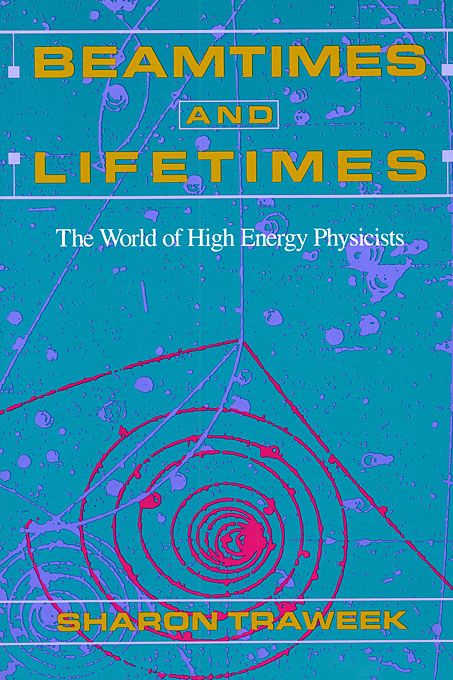
\includegraphics[width=\linewidth]{traweek-beamtimes-and-lifetimes.jpg}}
\end{columns}
\end{frame}

\begin{frame}{\only<1>{My expectation 6 years ago: Spark, Hadoop, functional big data}\only<2->{Completely changed by focus group/interview/survey feedback}}
\vspace{0.5 cm}
\begin{columns}
\column{1.12\linewidth}
\only<1>{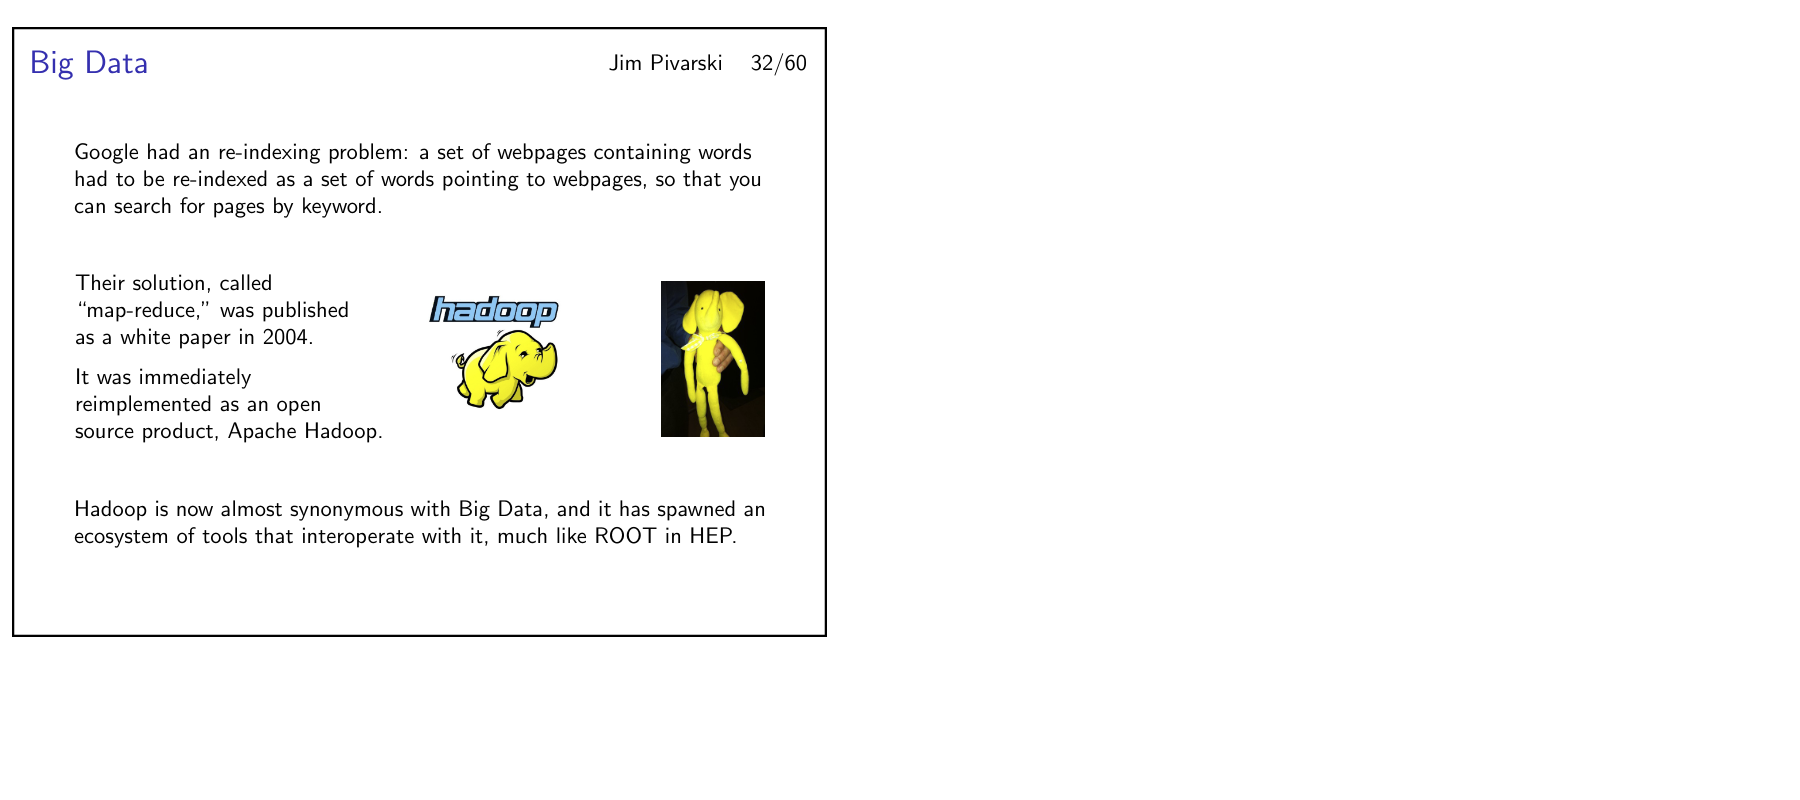
\includegraphics[width=\linewidth]{evolving-views-1.png}}\only<2>{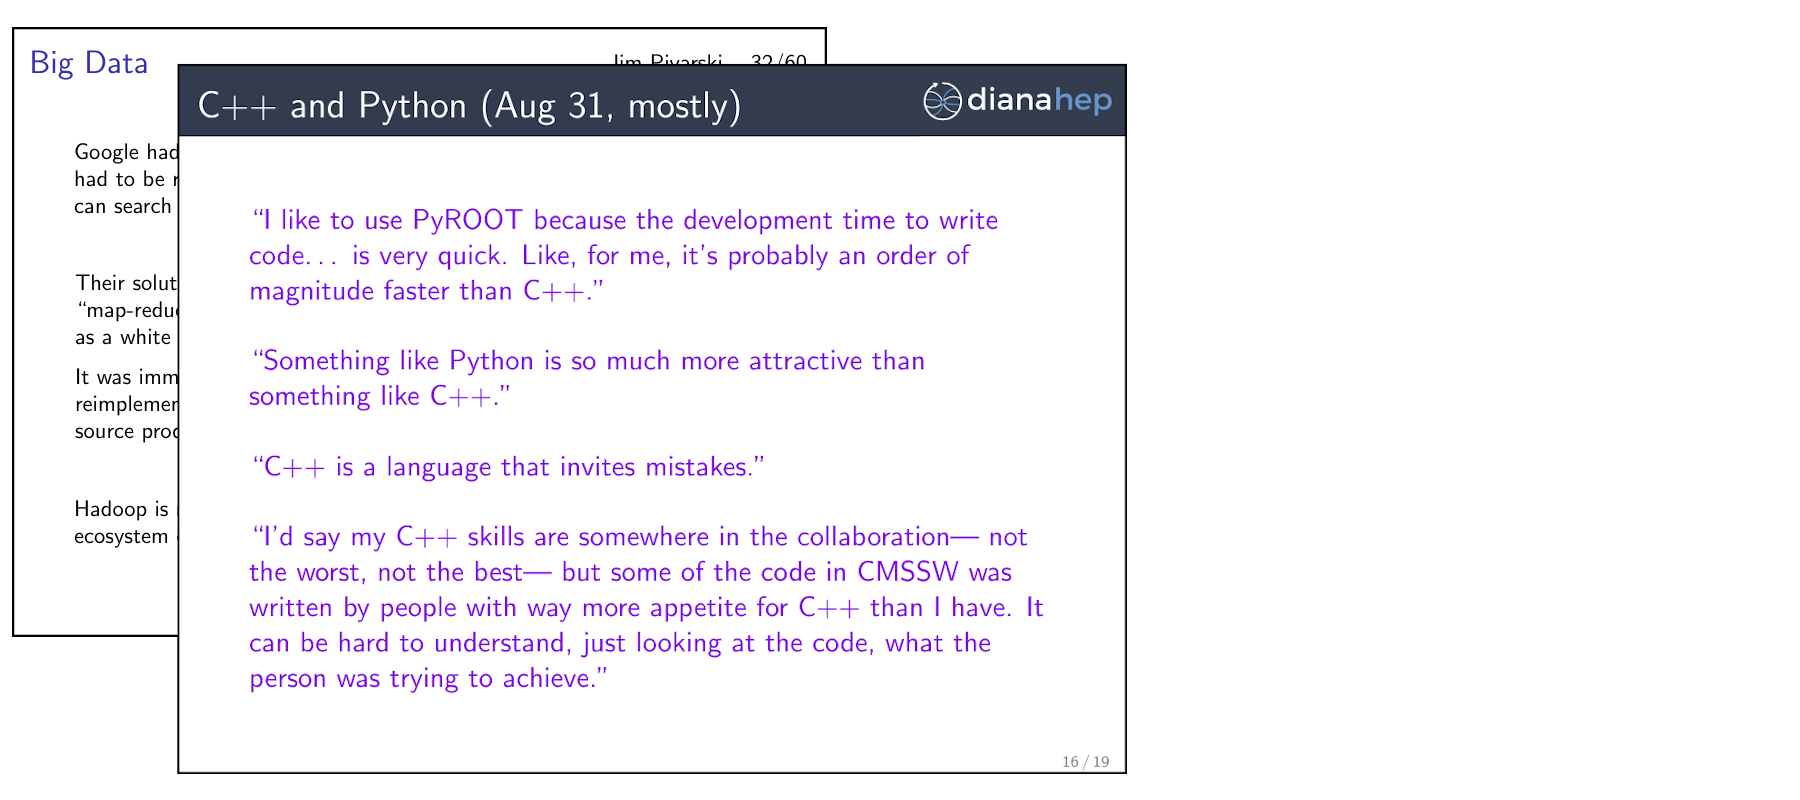
\includegraphics[width=\linewidth]{evolving-views-2.png}}\only<3>{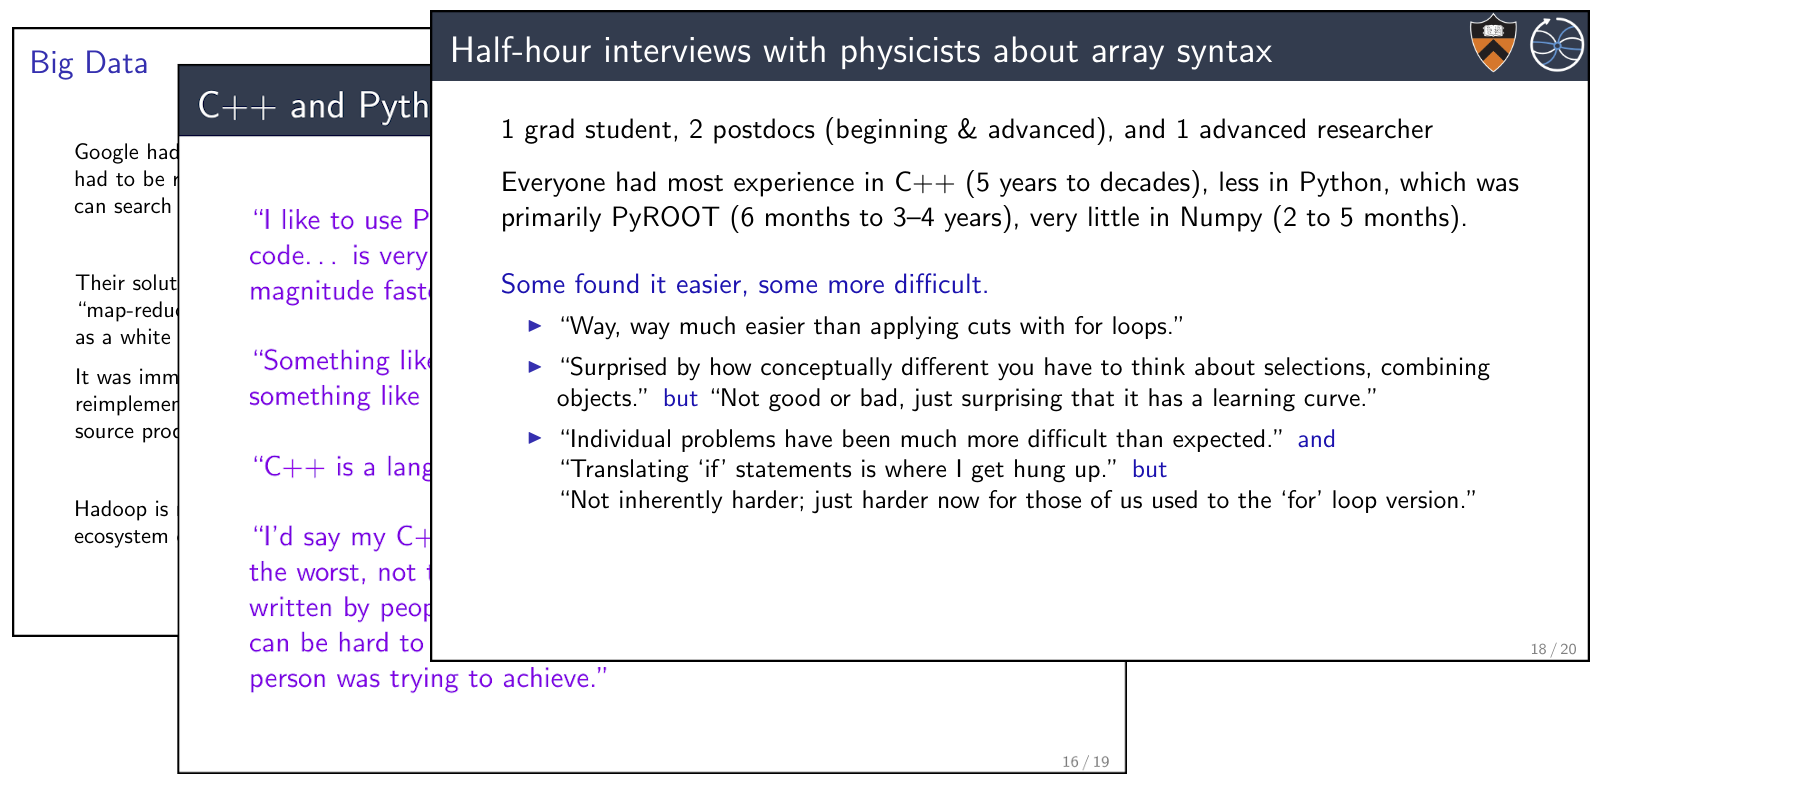
\includegraphics[width=\linewidth]{evolving-views-3.png}}\only<4>{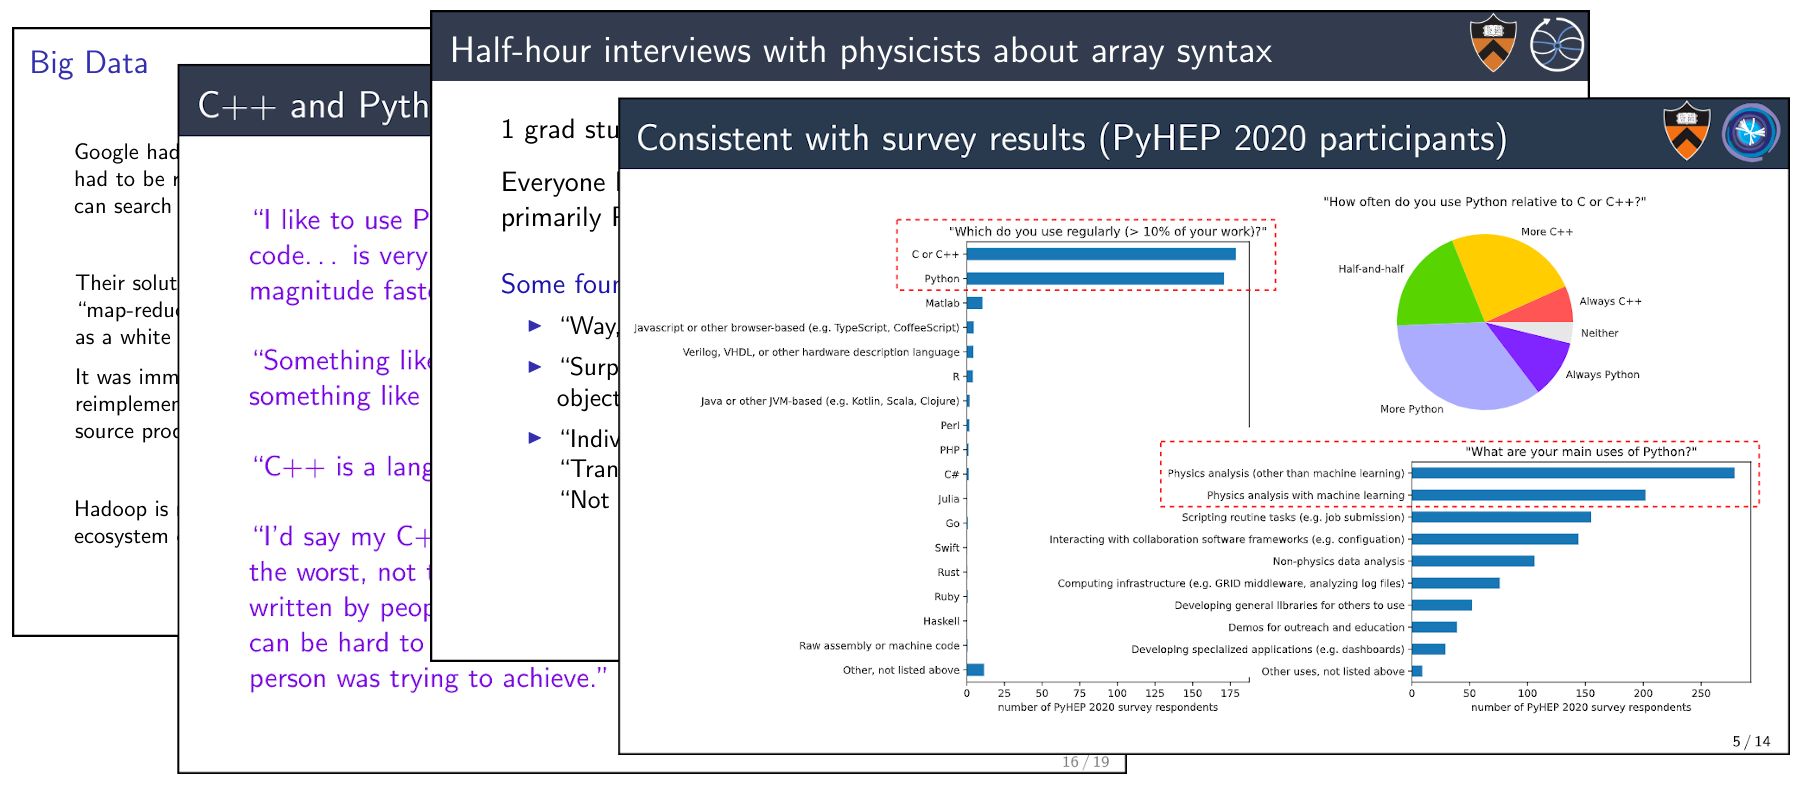
\includegraphics[width=\linewidth]{evolving-views-4.png}}
\end{columns}
\end{frame}

\begin{frame}{Ways to study humans}
\vspace{0.1 cm}
\textcolor{gray}{\scriptsize (Important note: I am not an expert. Below is what I learned from conversations with them.)}

\large
\vspace{0.1 cm}
\begin{itemize}\setlength{\itemsep}{0.25 cm}
\item<1-> \textcolor{darkblue}{Qualitative:}

\vspace{0.05 cm}
\begin{itemize}\large\setlength{\itemsep}{0.15 cm}
\item \textcolor{darkblue}{Focus groups:} \normalsize most open to unexpected ideas. Want to keep the group size and mix such that participants are willing to speak up. Goal is to discover new {\it dimensions} of the vector space, not just points within it. \large

\item \textcolor{darkblue}{One-on-one interviews:} \normalsize can be deeper but less broad than focus groups. Lacks the multiplying effect of responding to each other's opinions. \large

\item \textcolor{darkblue}{History/documents:} \normalsize observational, rather than experimental, but this method can reach further into the past. \large
\end{itemize}

\item<2-> \textcolor{darkblue}{Quantitative:}

\vspace{0.05 cm}
\begin{itemize}\large\setlength{\itemsep}{0.15 cm}
\item \textcolor{darkblue}{Surveys:} \normalsize can get large, statistically meaningful datasets, at the cost of losing flexibility/openness to new ideas. Now you {\it are} filling in a vector space. \large

\item \only<2>{\fcolorbox{white}{white}{\textcolor{darkblue}{Proxy metrics:} \normalsize can measure what people {\it do}, rather than what they {\it say}.}}\only<3>{\fcolorbox{black}{lightyellow}{\textcolor{darkblue}{Proxy metrics:} \normalsize can measure what people {\it do}, rather than what they {\it say}.}} \large
\end{itemize}

\end{itemize}

\vspace{10 cm}
\end{frame}

\begin{frame}{Proxy metrics: high statistics, cautious interpretation}
\vspace{0.25 cm}
\mbox{\hspace{0.75 cm}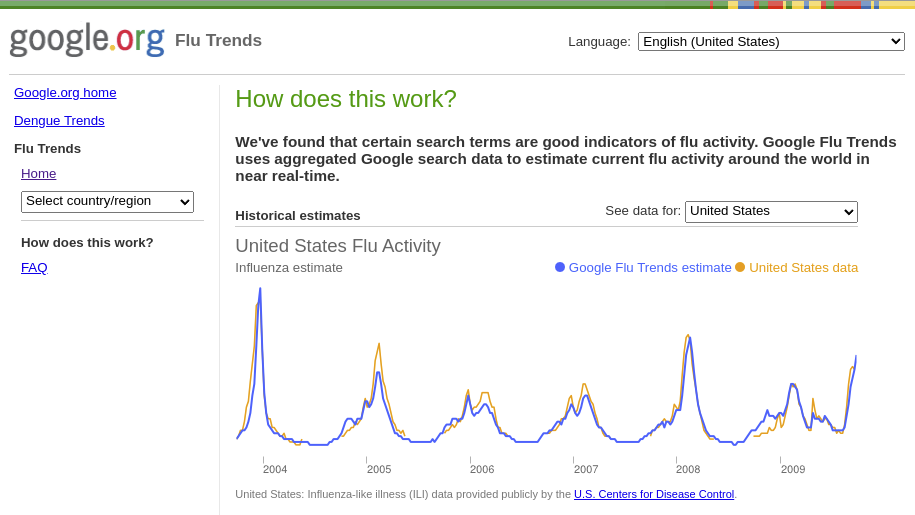
\includegraphics[width=\linewidth]{google-flu-trends.png}}

\begin{uncoverenv}<2->
\vspace{-3.35 cm}
\hspace{-0.25 cm}\begin{minipage}{0.3\linewidth}
{\bf Google Flu Trends}

{\bf (2008--2015)}

\small
\vspace{0.25 cm}
Count searches for

things like ``fever,'' ``cough,''

interpret as flu activity.

\vspace{0.25 cm}
(This was controversial.)
\end{minipage}
\vspace{3.35 cm}
\end{uncoverenv}
\end{frame}

\begin{frame}{Example: what happened here?}
\vspace{0.25 cm}
\textcolor{darkblue}{\mbox{\hspace{-0.5 cm}}Number of stars on Awkward Array's GitHub repo versus time}

\vspace{0.25 cm}
\begin{columns}
\column{0.75\linewidth}
% \only<1-2>{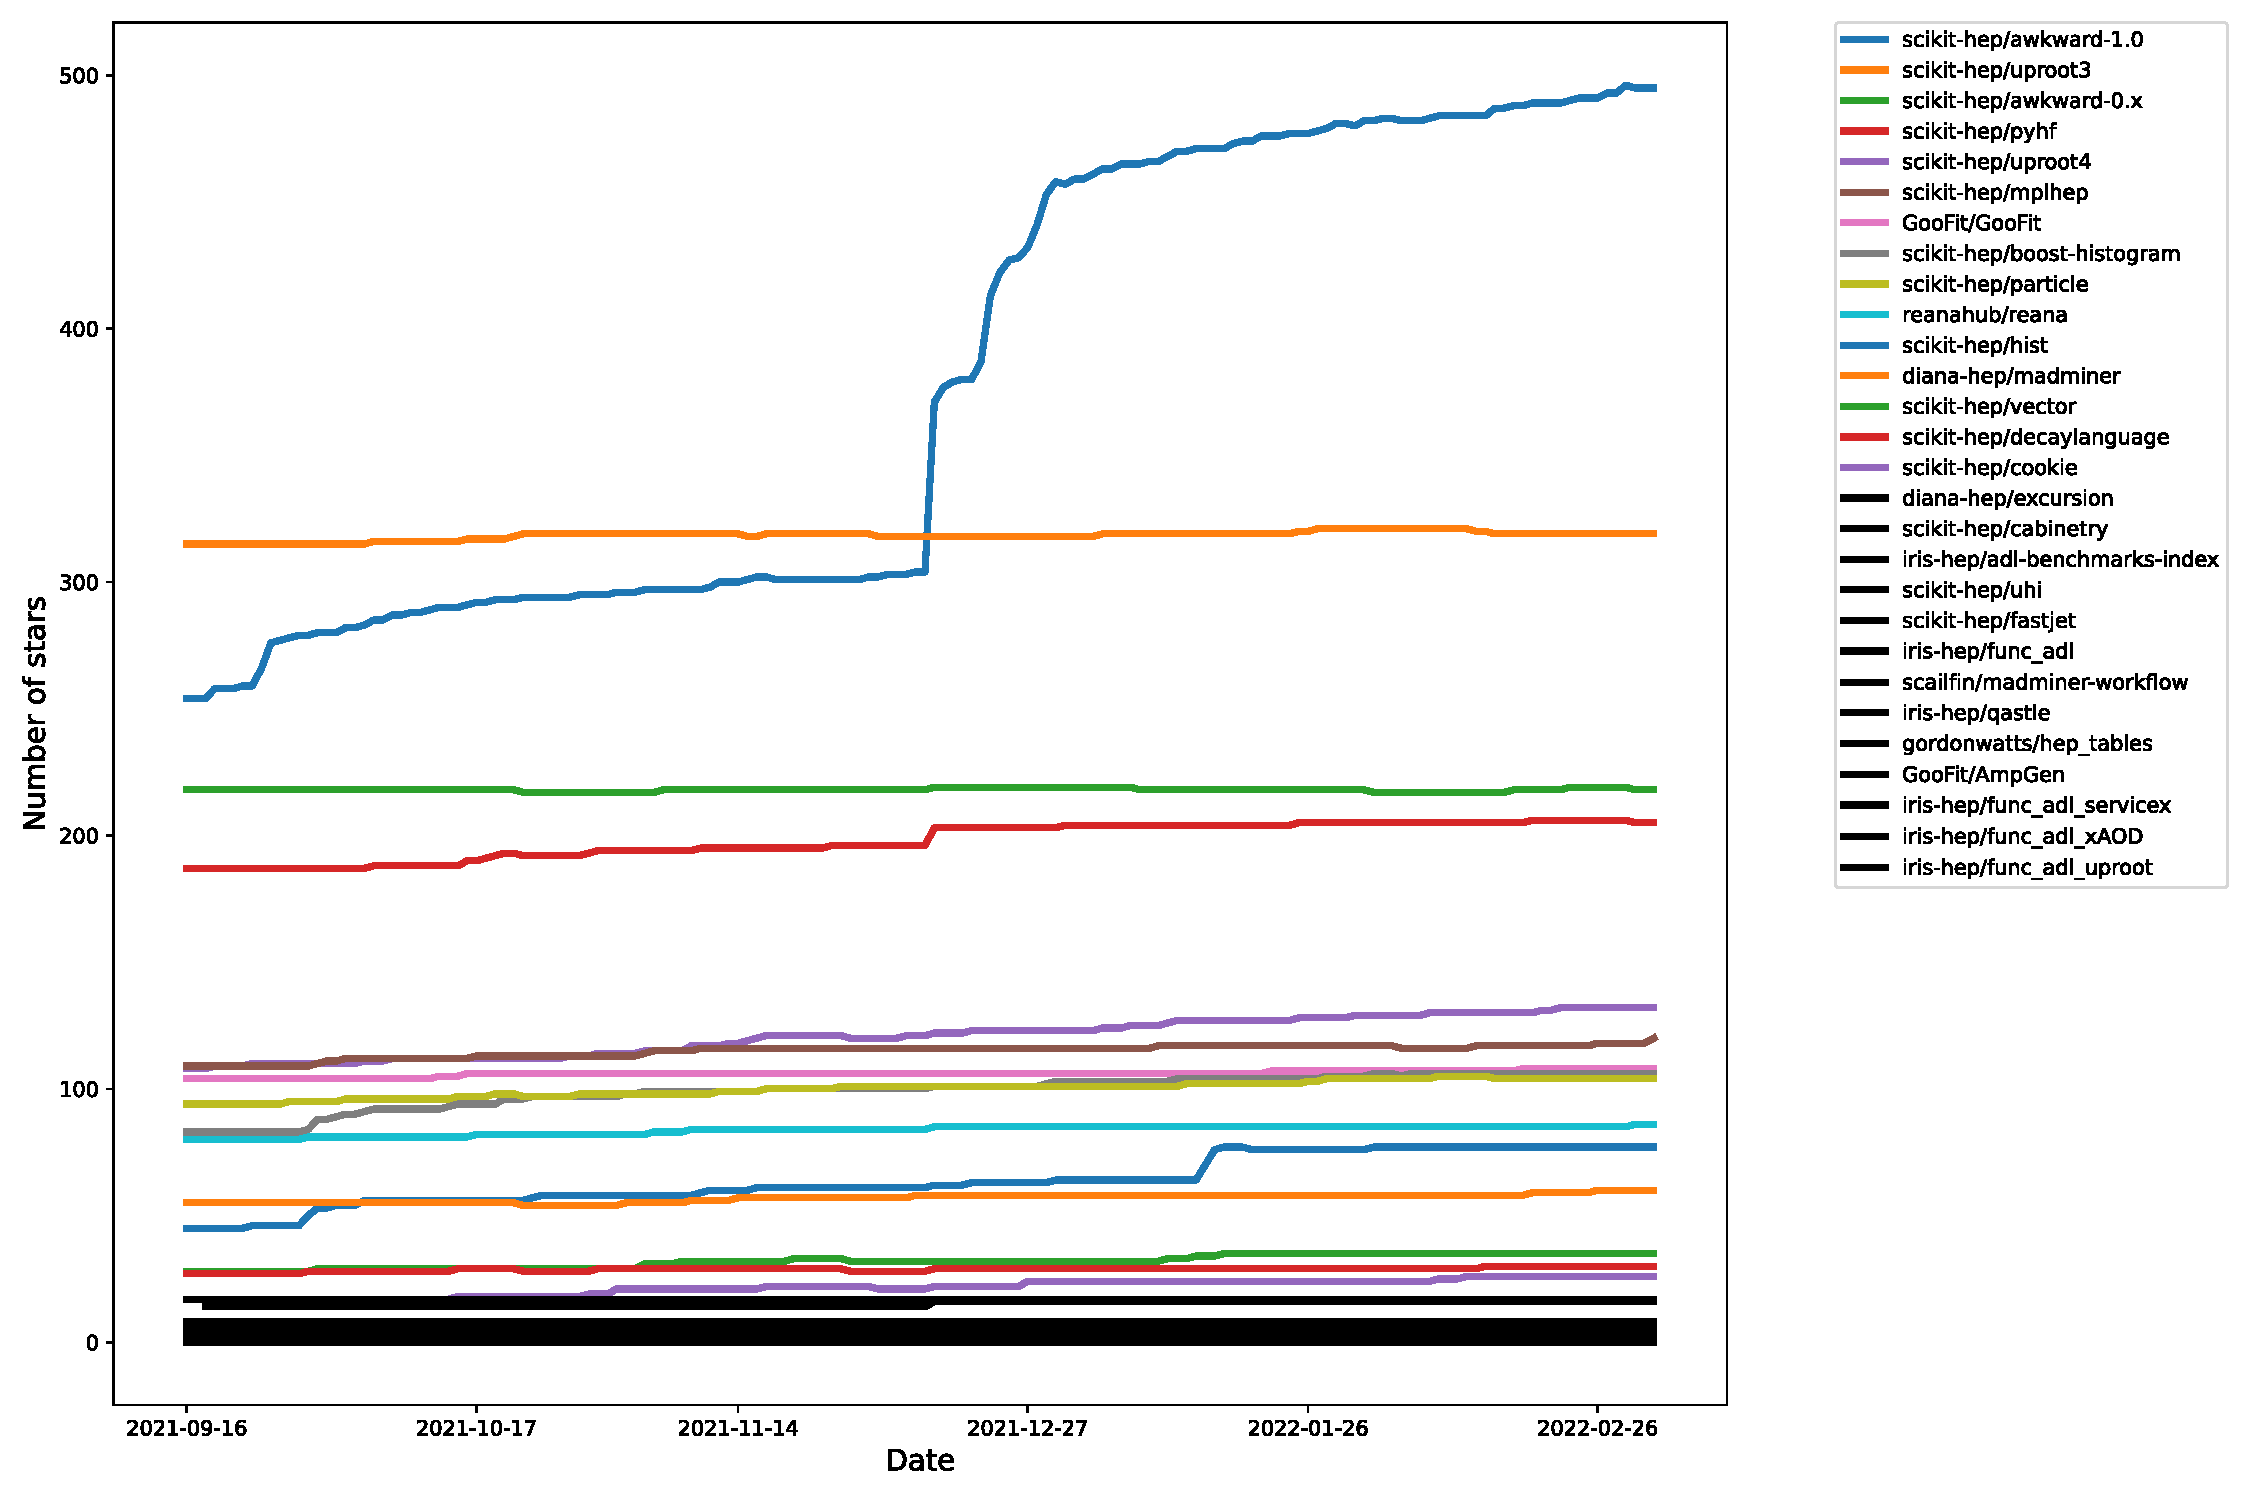
\includegraphics[width=\linewidth]{irishep-as-stars-1.pdf}}\only<3->{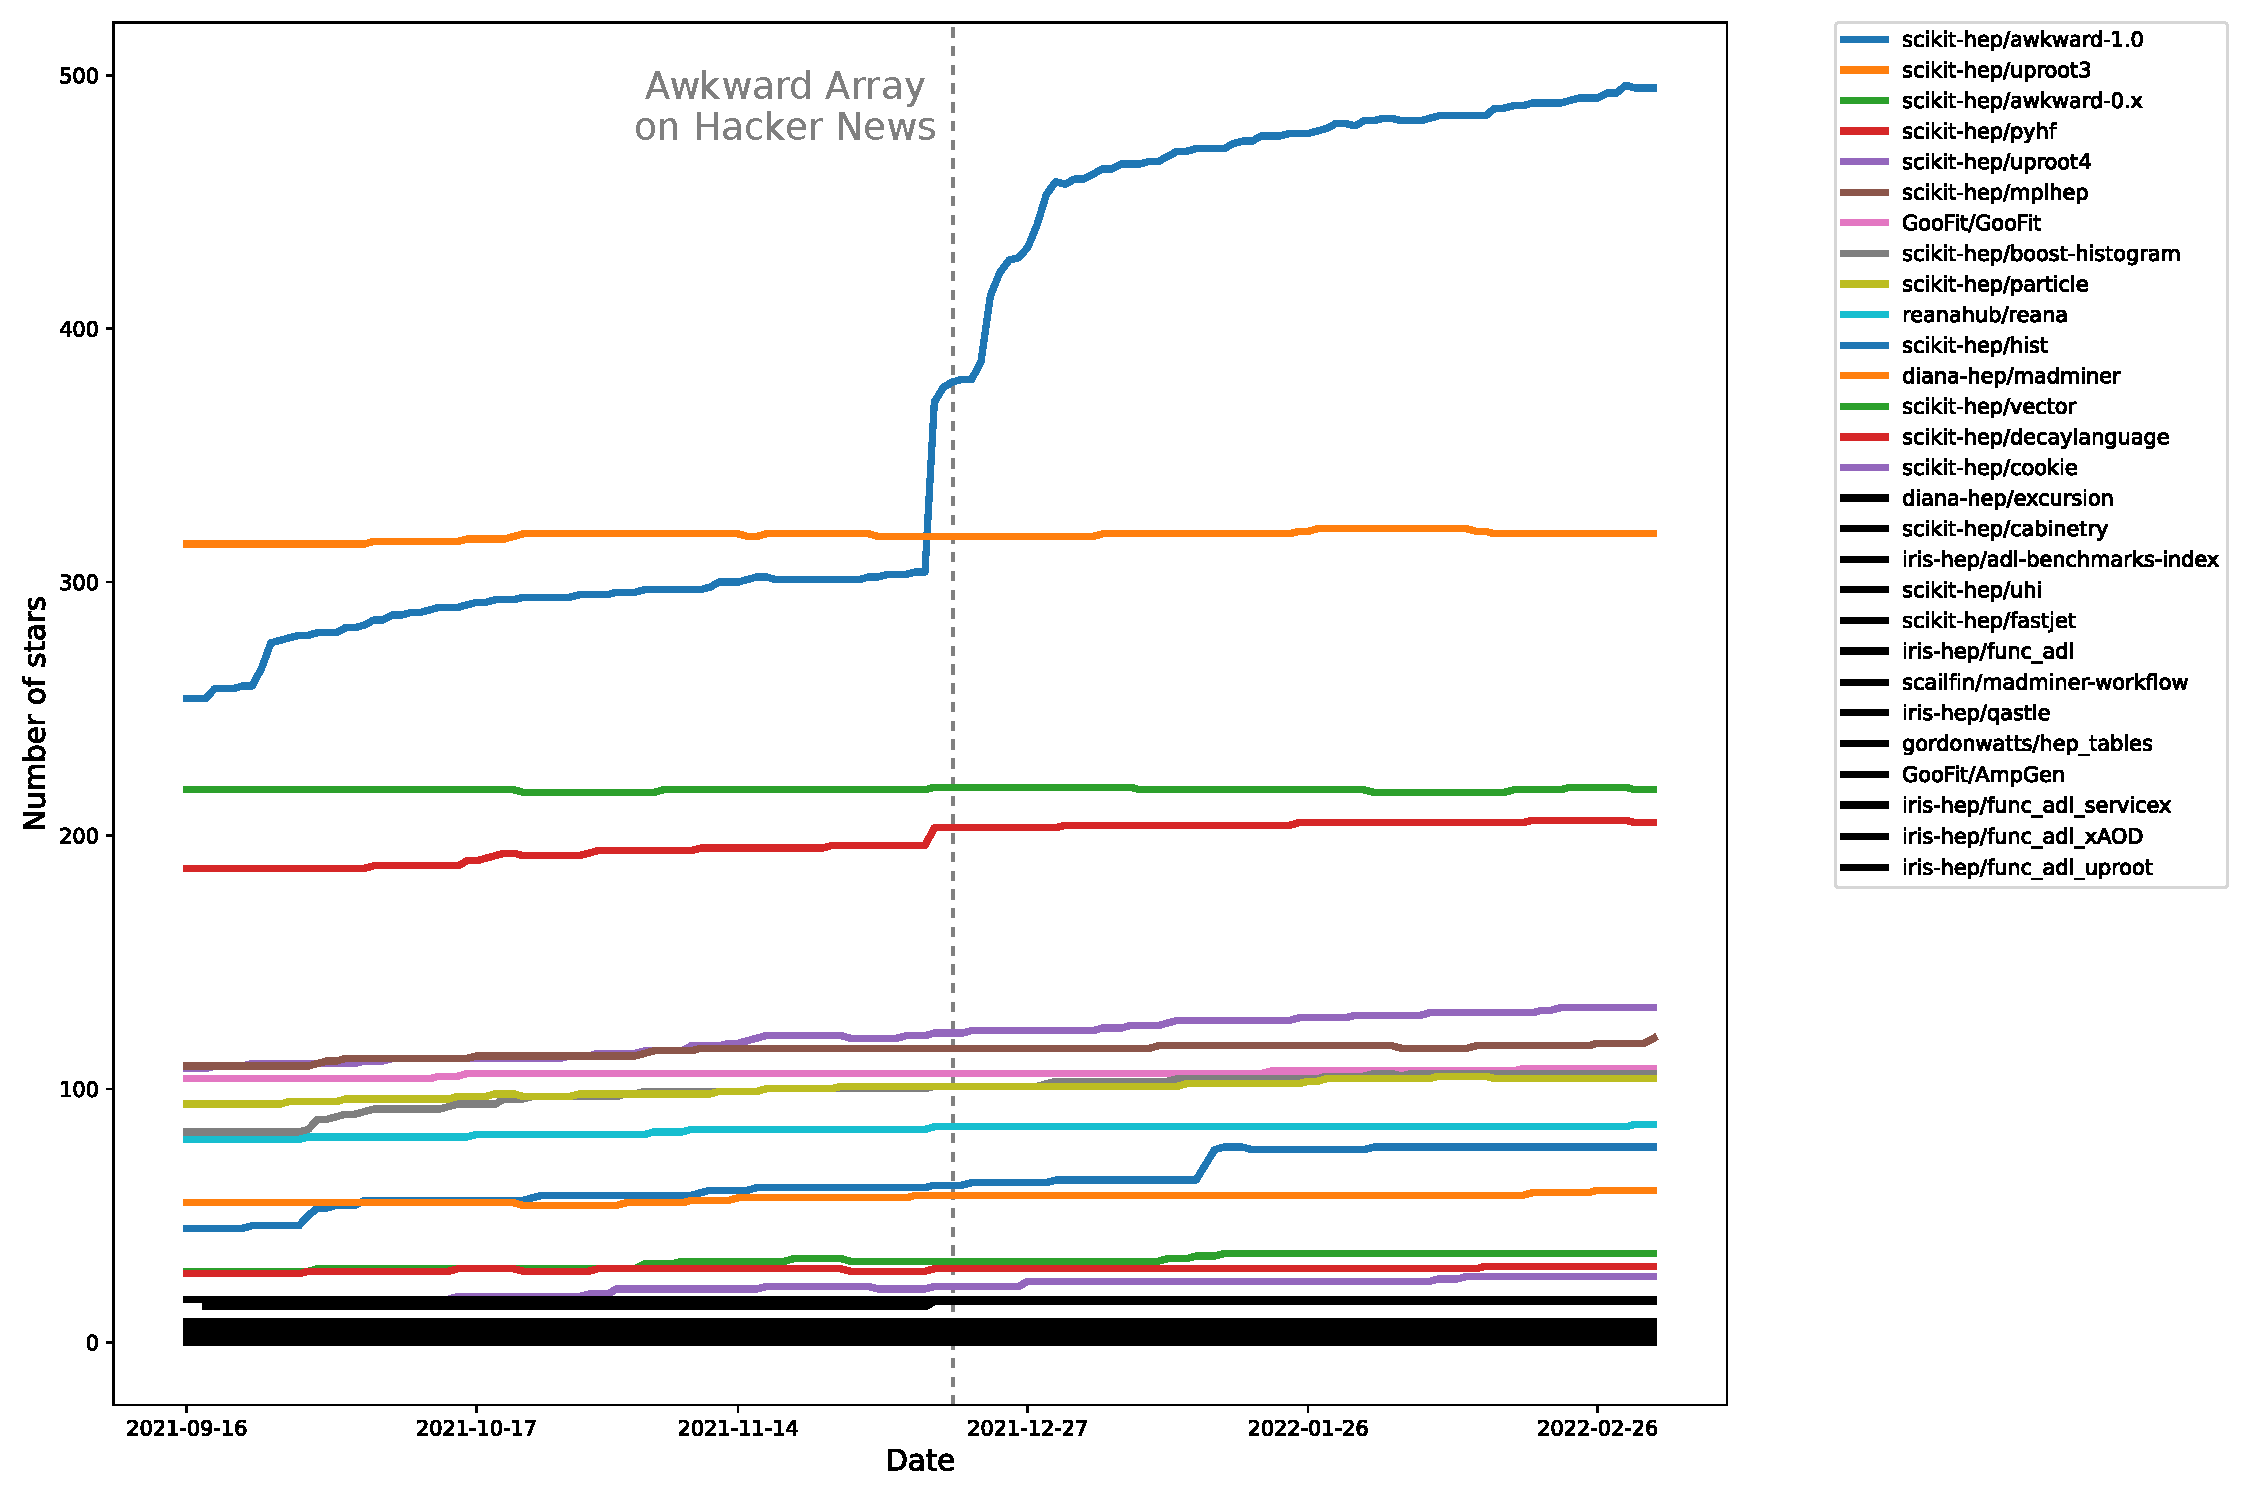
\includegraphics[width=\linewidth]{irishep-as-stars-2.pdf}}
\only<1-2>{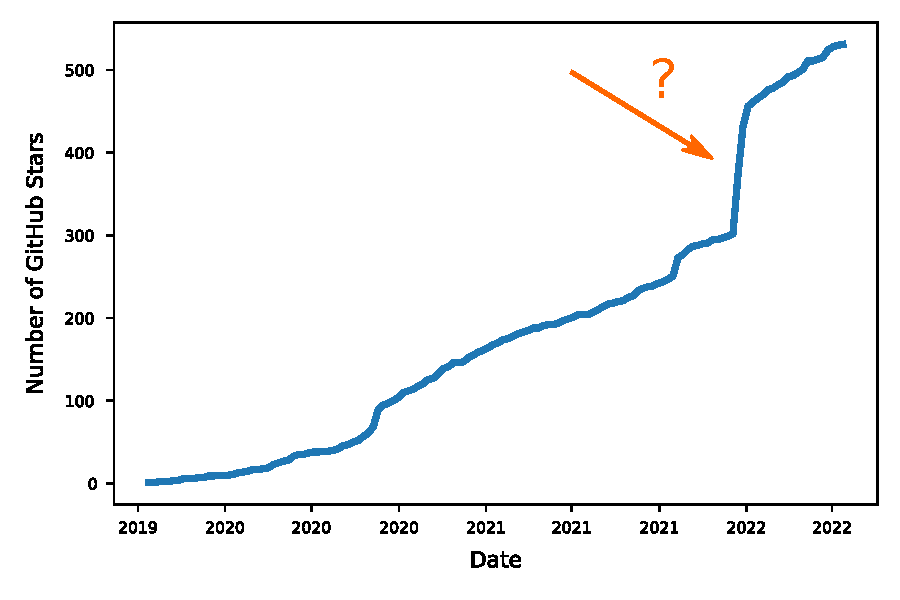
\includegraphics[width=\linewidth]{irishep-as-stars-3-before.pdf}}\only<3->{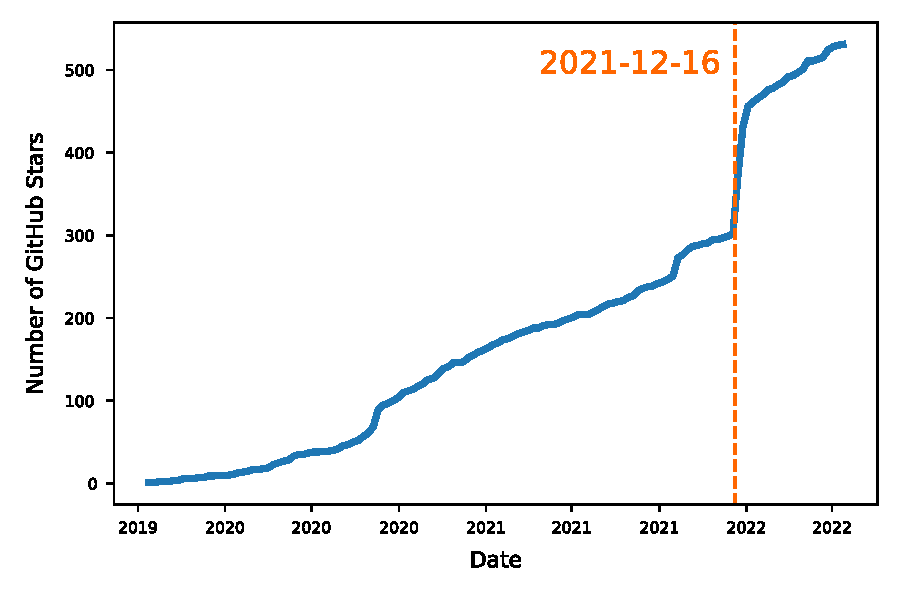
\includegraphics[width=\linewidth]{irishep-as-stars-3.pdf}}

\column{0.25\linewidth}
\uncover<2->{What we're trying to explain is a big, qualitative feature, not the little bumps.}

\vspace{0.2 cm}
\uncover<3->{Temporally coincides with Awkward Array on Hacker News:}

\uncover<3->{\small\textcolor{blue}{\url{https://news.ycombinator.com/item?id=29576323}}}

\vspace{0.2 cm}\normalsize
\uncover<4->{It shouldn't be too controversial to call a correlation like this ``causal.''}

\vspace{0.5 cm}
\end{columns}
\end{frame}

\begin{frame}{\mbox{ }}
\vspace{1 cm}
\begin{center}
\Large What about counting downloads (a traditionally favorite metric)?
\end{center}
\end{frame}

\begin{frame}{Stacked download statistics for Scikit-HEP and related packages}
\vspace{-0.25 cm}
\begin{columns}
\column{1.2\linewidth}
\mbox{\hspace{-1 cm}\only<1>{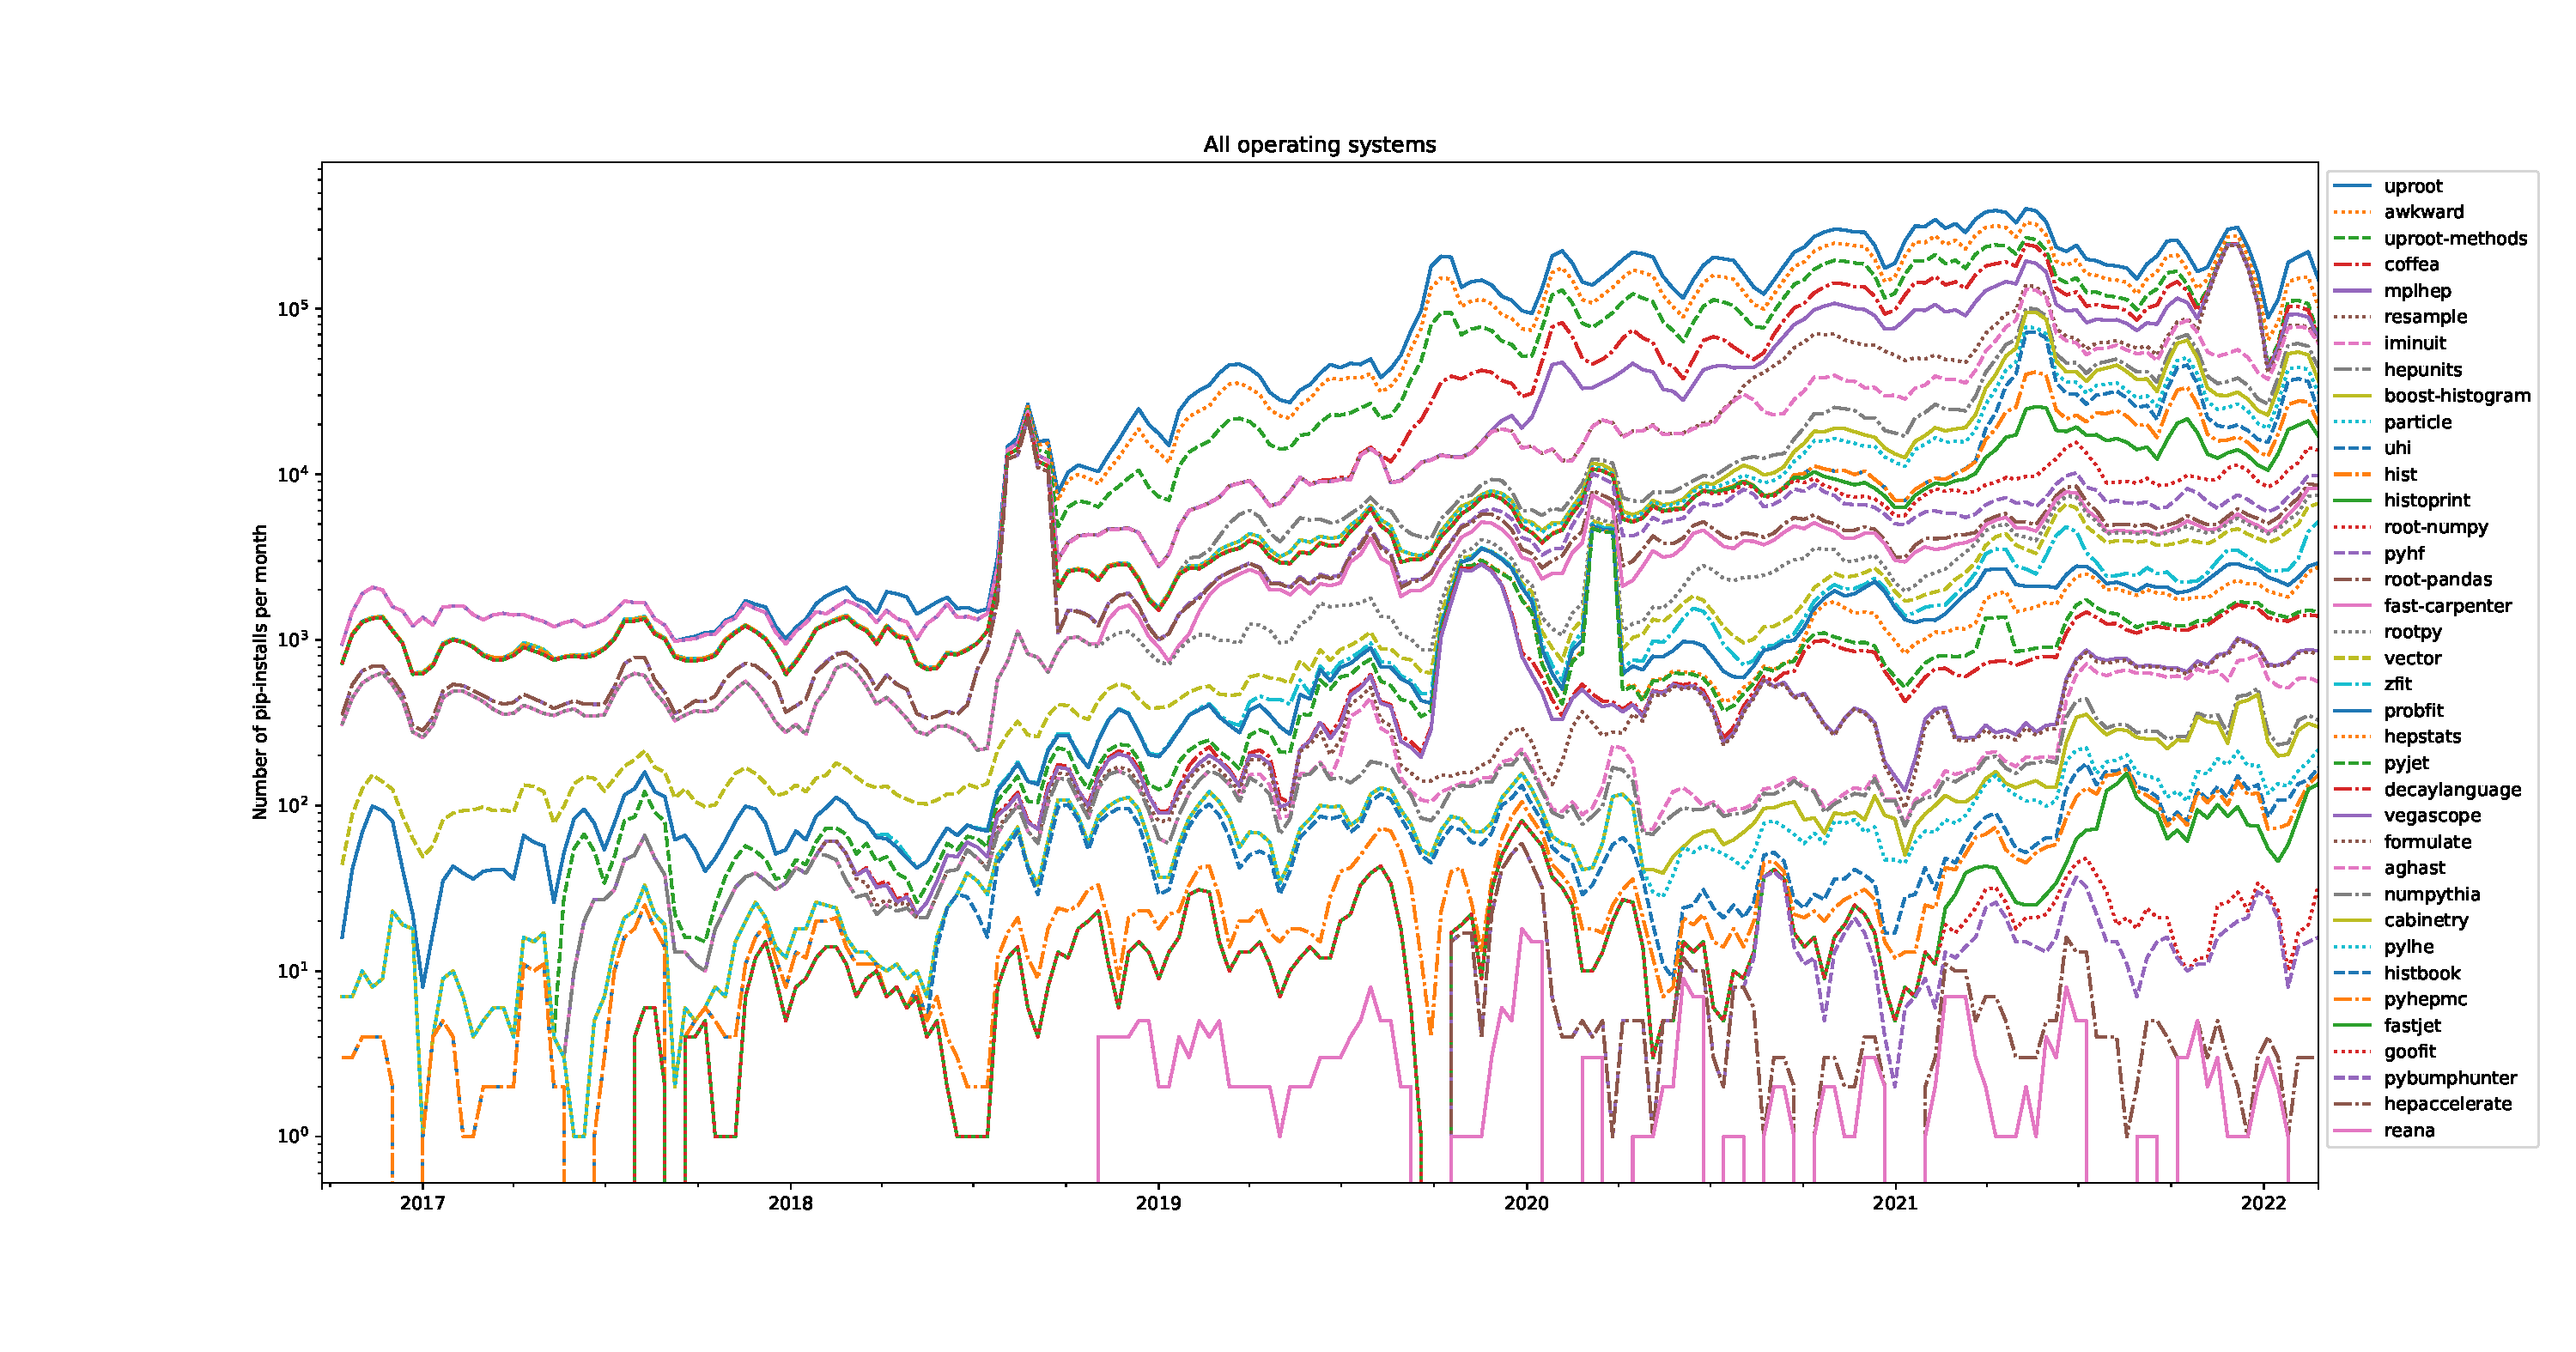
\includegraphics[width=\linewidth]{pip-allos-scikithep-log.pdf}}\only<2>{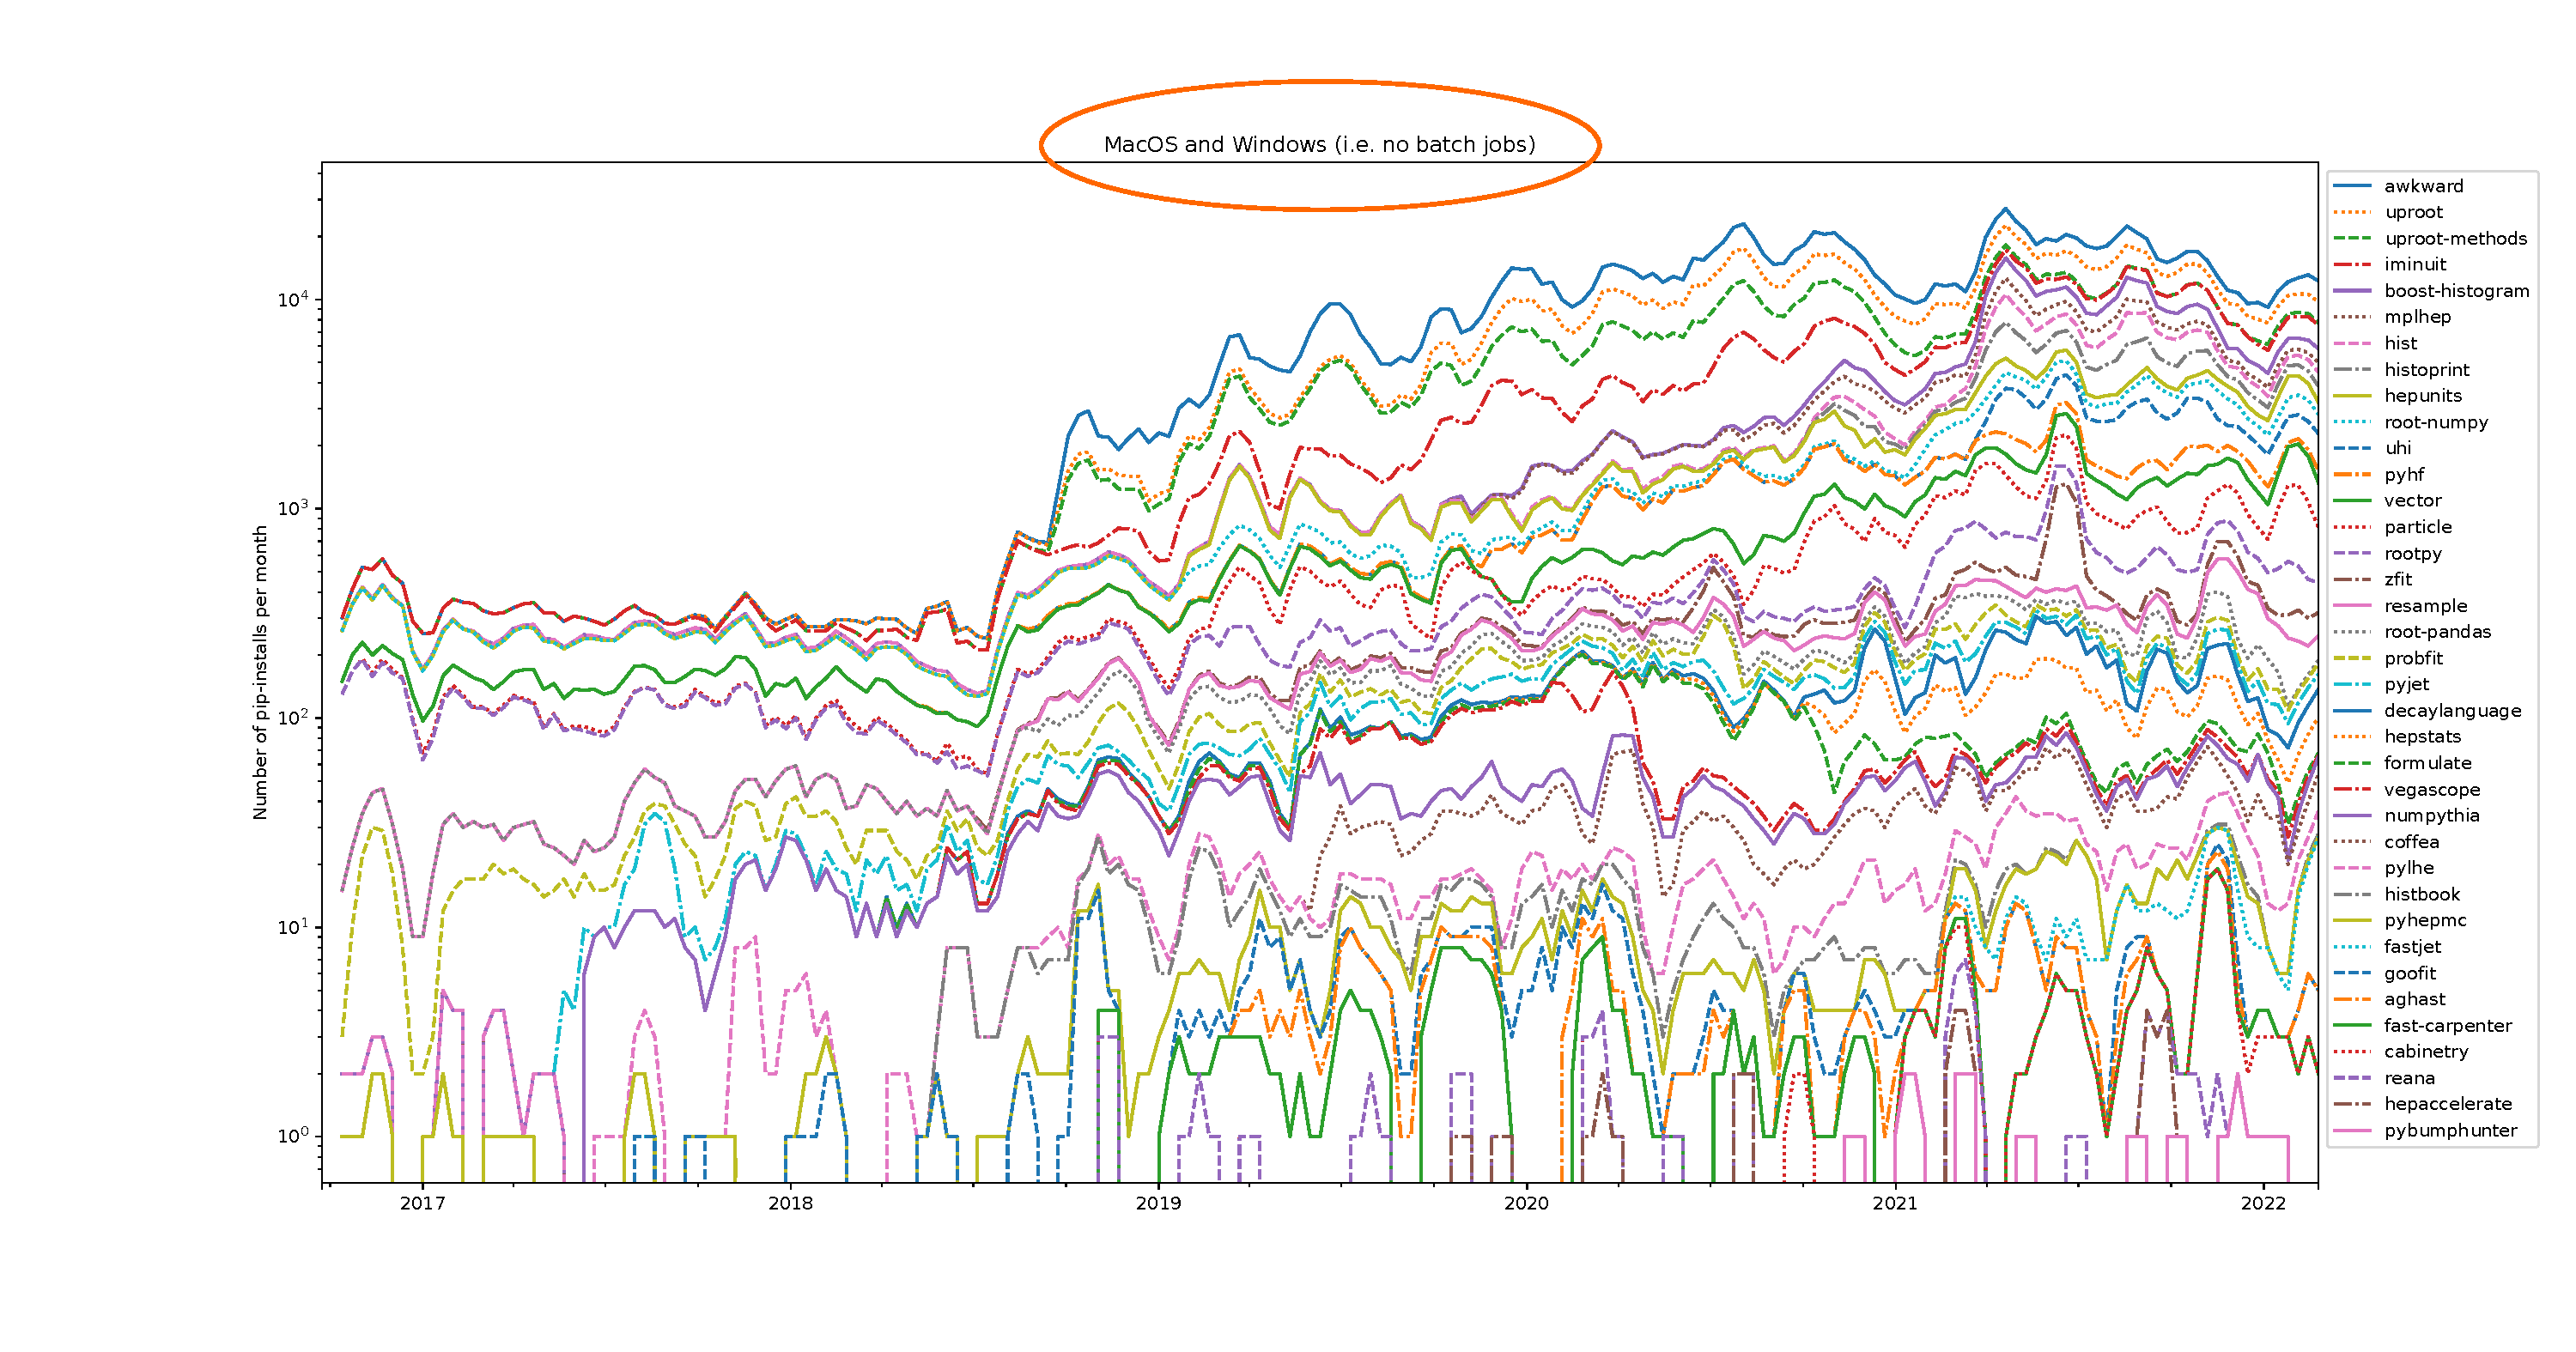
\includegraphics[width=\linewidth]{pip-macwin-scikithep-log.pdf}}}
\end{columns}
\end{frame}

\begin{frame}{\mbox{ }}
\Large
\vspace{0.4 cm}

Linux includes batch jobs, which sometimes \mintinline{bash}{pip install} the same package on thousands of workers.

\vspace{0.5 cm}
\uncover<2->{Selecting only MacOS and Windows removes most batch jobs, but it excludes some individual users (like me), probably with a behavioral bias.}

\vspace{0.5 cm}
\uncover<3->{Still, there's continuous testing jobs on MacOS and Windows.}

\vspace{0.5 cm}
\uncover<4->{Do we even {\it want} to exclude these things? What do we {\it want} the observable to quantify?}
\end{frame}

%% \begin{frame}{How about this one: Python version in \only<1-2>{\mintinline{bash}{pip install uproot}}\only<3-4>{\mintinline{bash}{pip install numpy}}}
%% \vspace{-0.25 cm}
%% \begin{columns}
%% \column{1.2\linewidth}
%% \only<1>{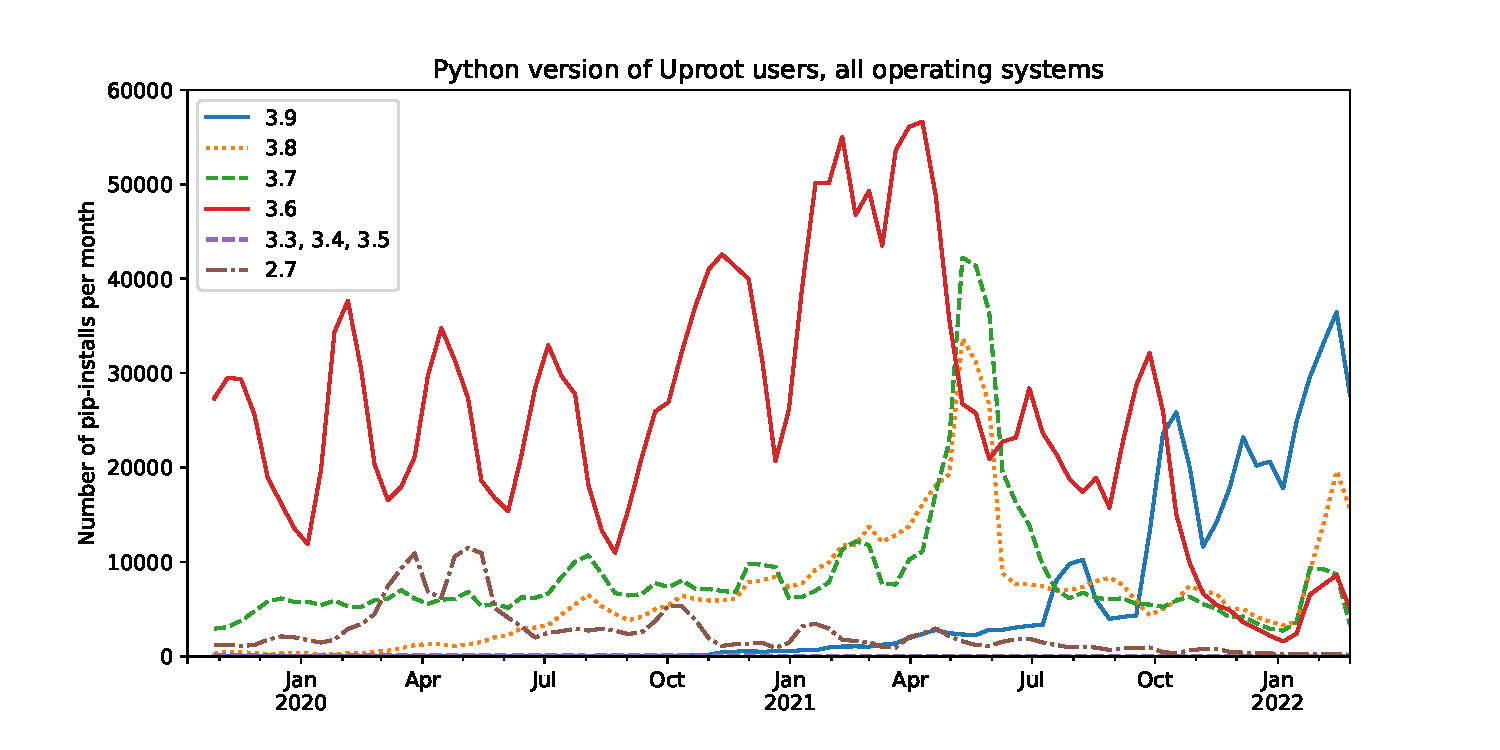
\includegraphics[width=\linewidth]{pip-allos-pythonversion-uprootusers-lin.pdf}}\only<2>{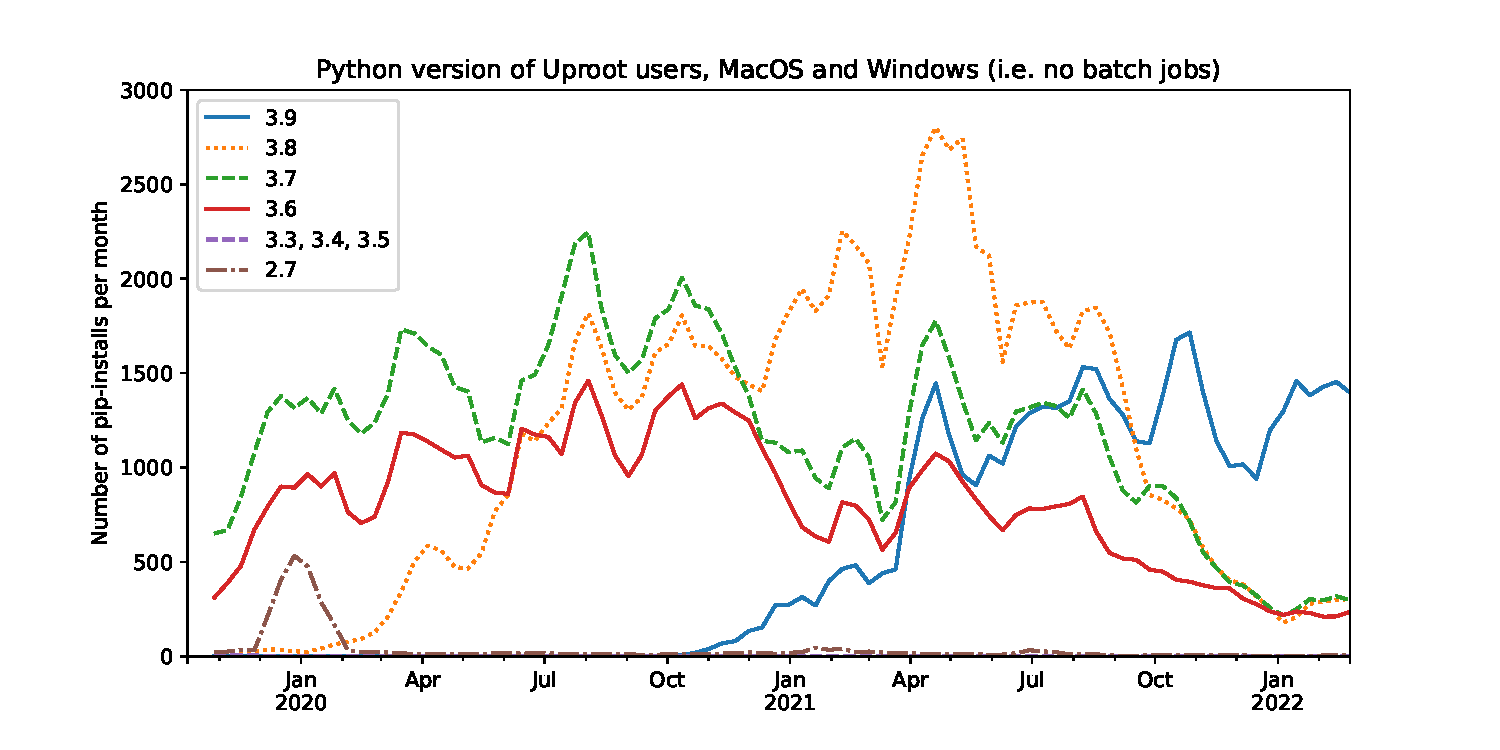
\includegraphics[width=\linewidth]{pip-macwin-pythonversion-uprootusers-lin.pdf}}\only<3>{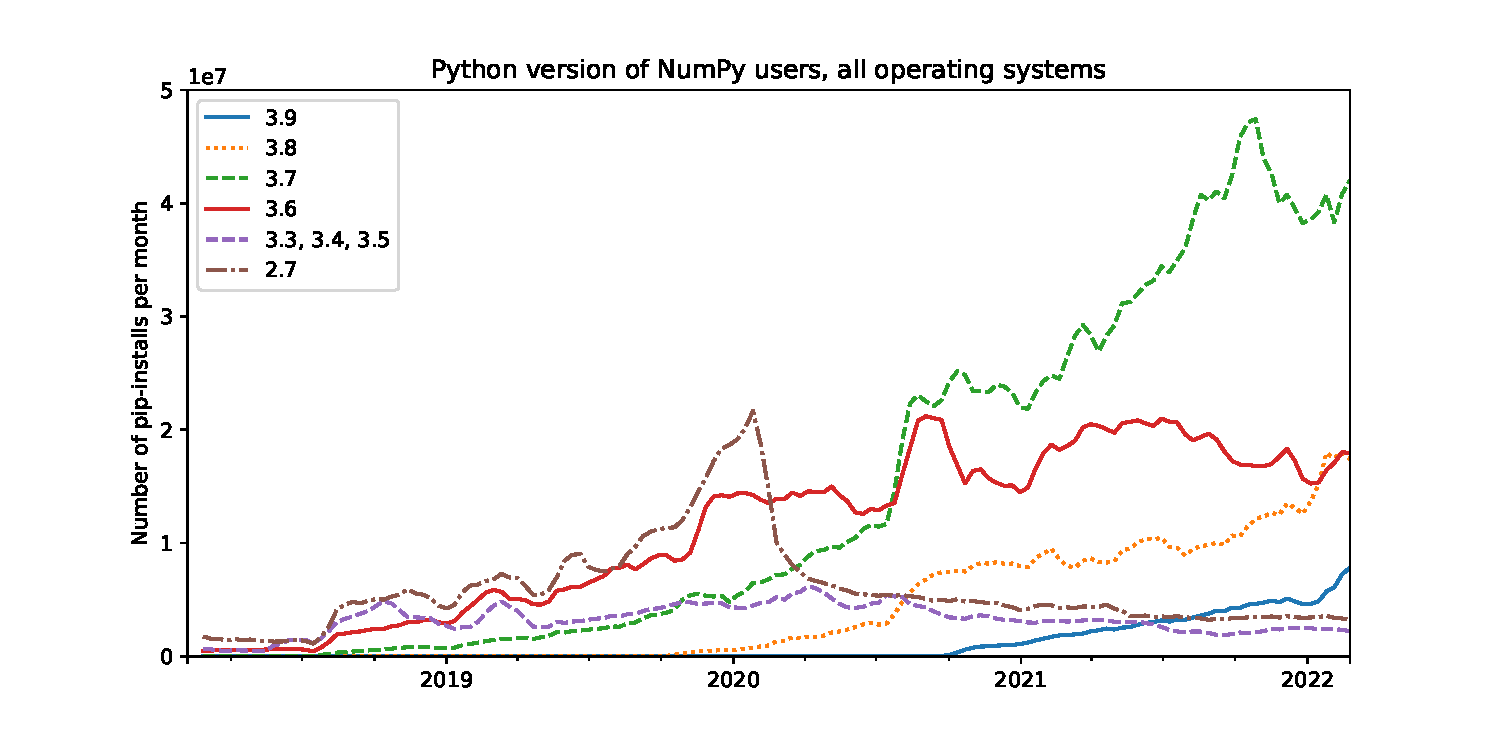
\includegraphics[width=\linewidth]{pip-allos-pythonversion-numpyusers-lin.pdf}}\only<4>{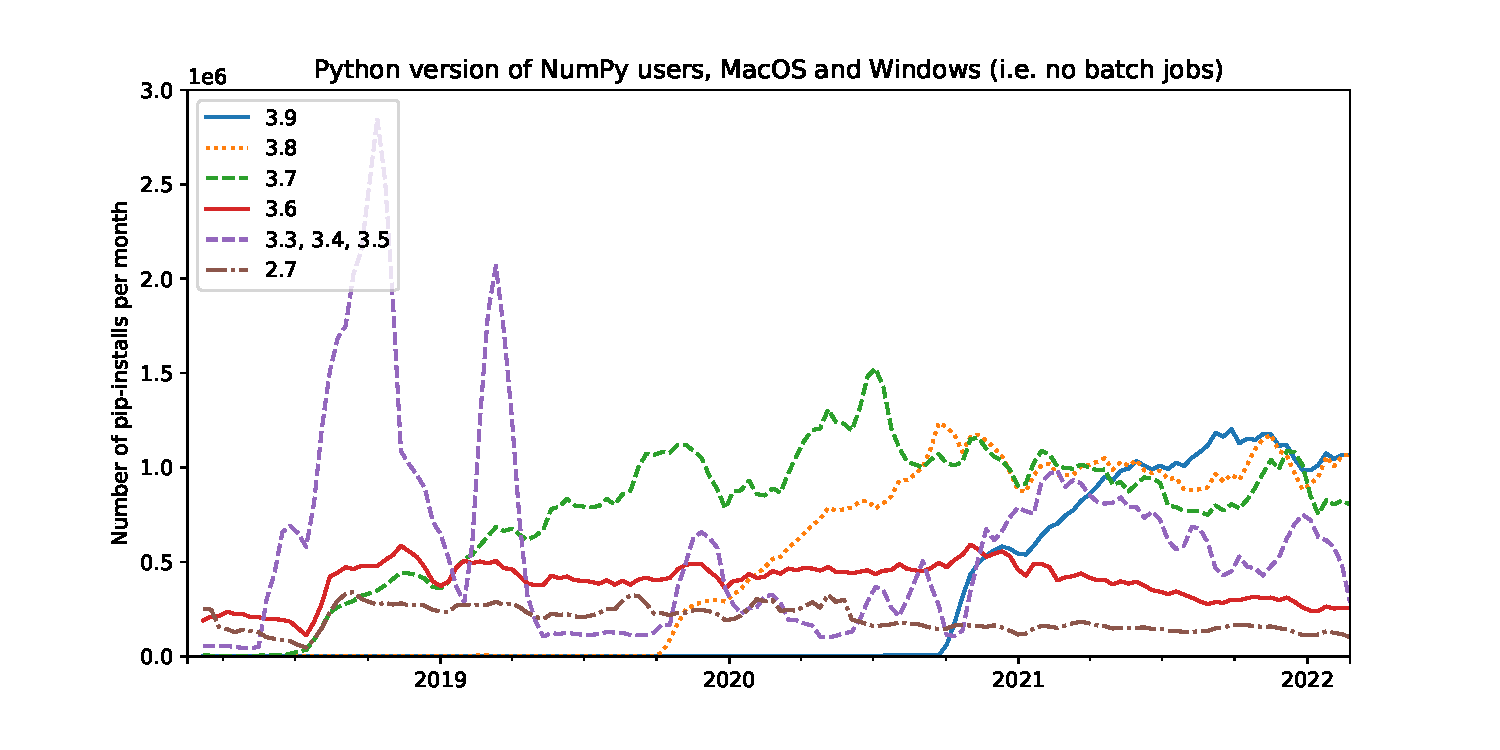
\includegraphics[width=\linewidth]{pip-macwin-pythonversion-numpyusers-lin.pdf}}
%% \end{columns}
%% \end{frame}

\begin{frame}{More often useful when {\it comparing} two things}
\vspace{0.25 cm}
\Large
\underline{Transition from ``old'' \only<1>{Uproot}\only<2>{Awkward} to ``new''}

\begin{center}
\only<1>{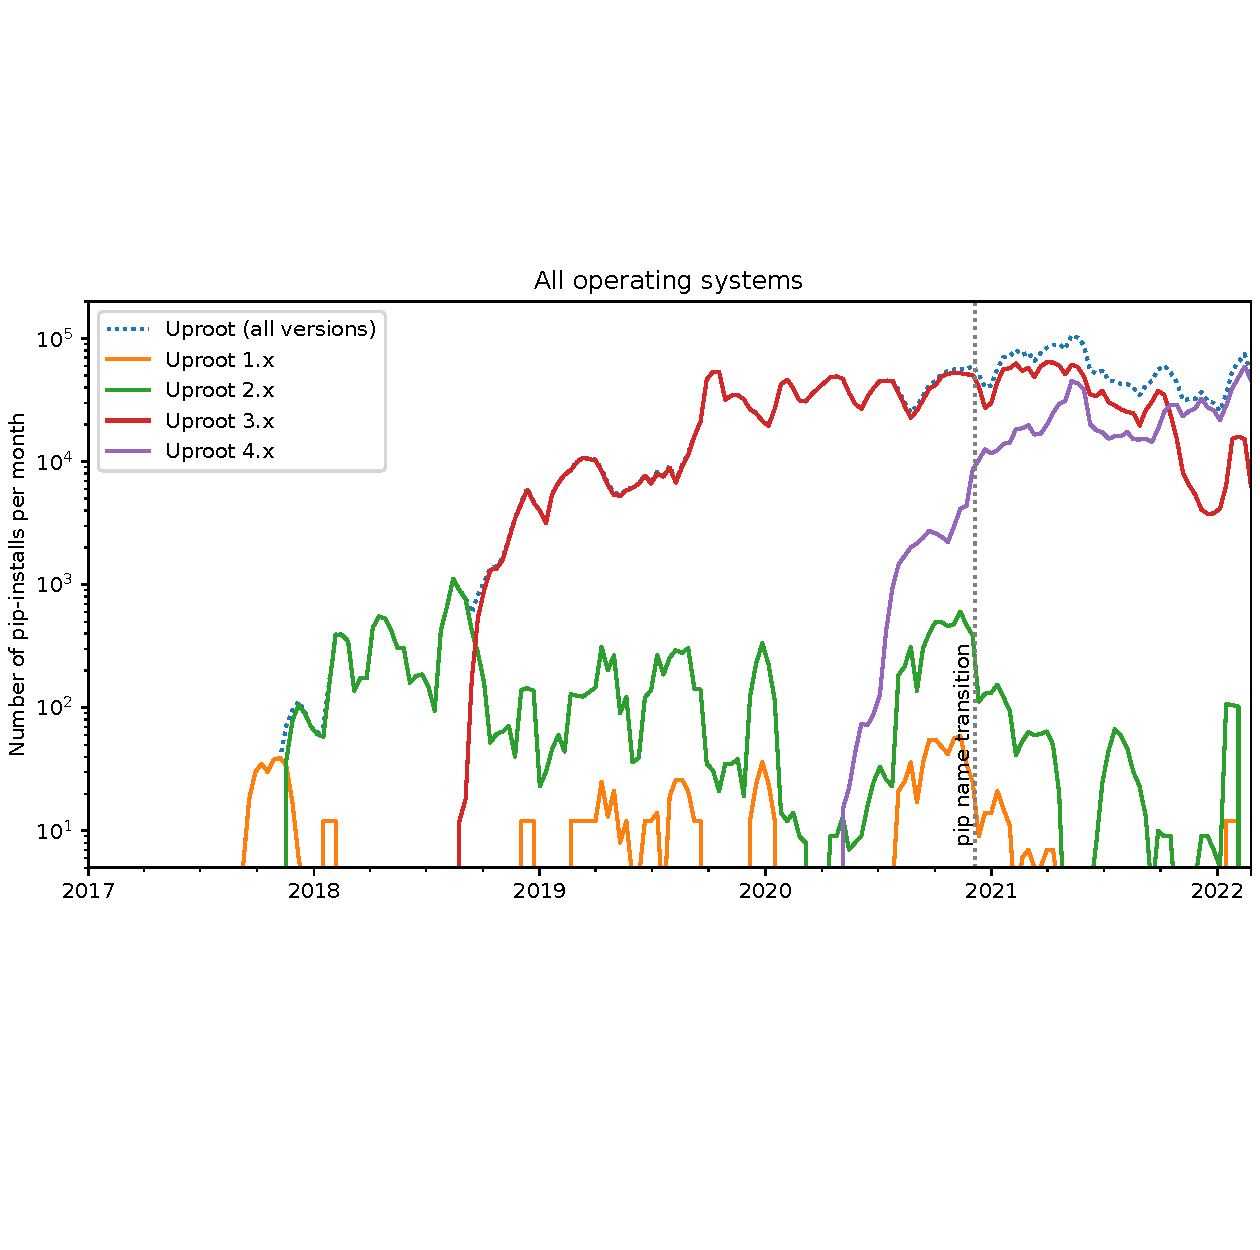
\includegraphics[width=0.9\linewidth]{pip-allos-uproot-log.pdf}}\only<2>{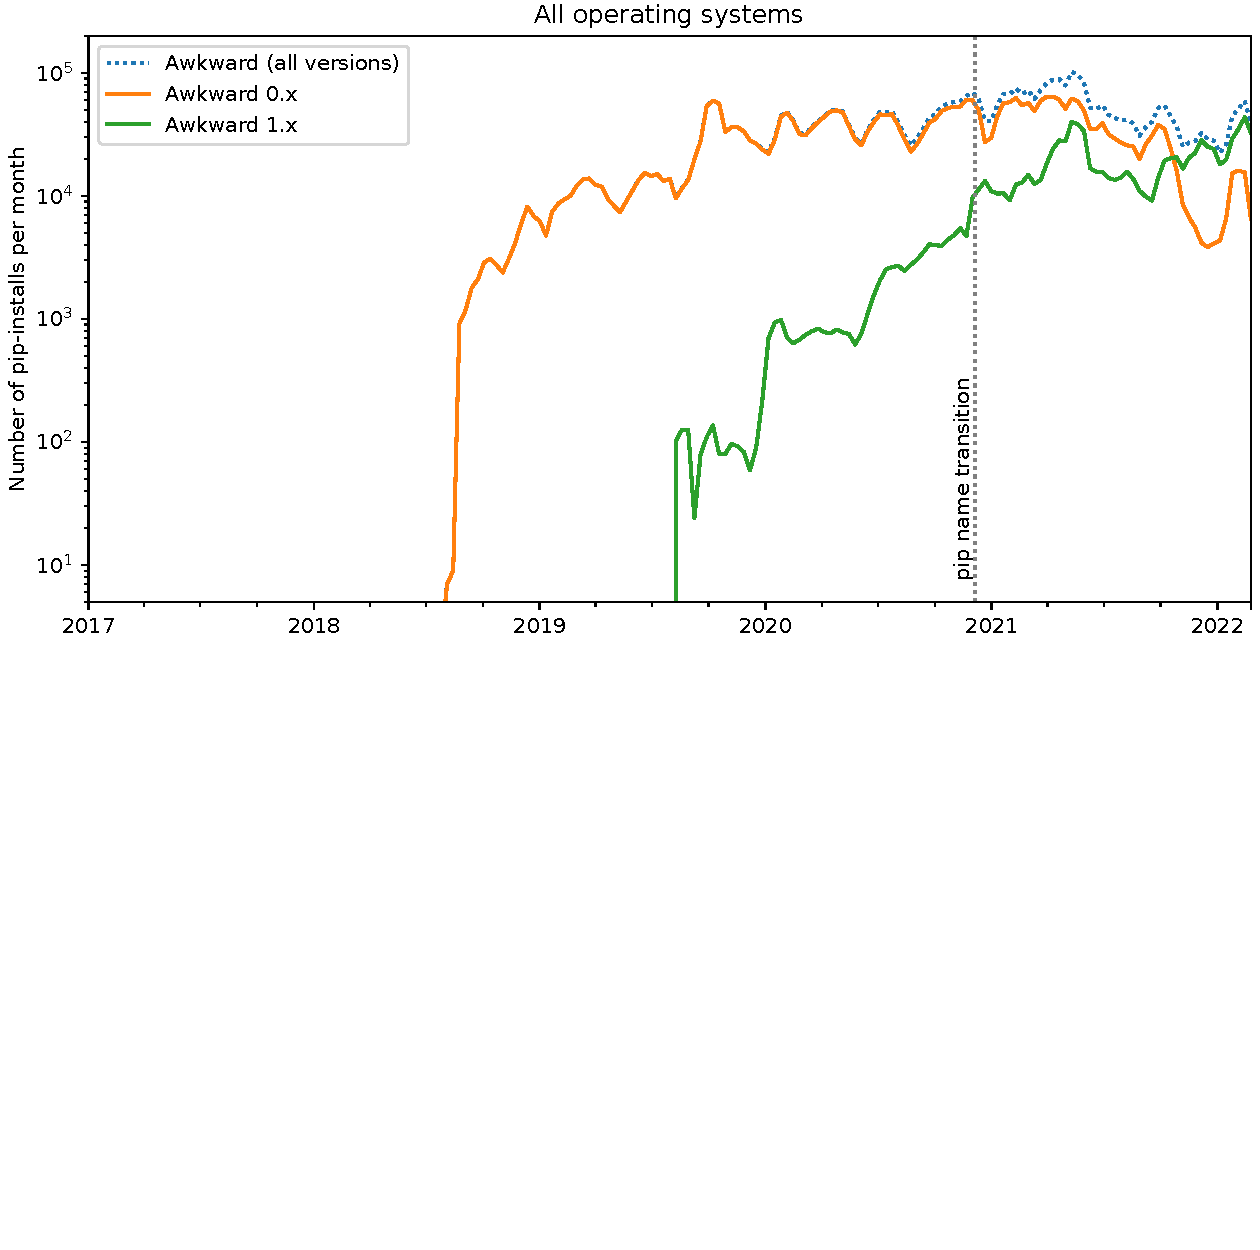
\includegraphics[width=0.9\linewidth]{pip-allos-awkward-log.pdf}}
\end{center}
\end{frame}

\begin{frame}{Directed study: how are physicists using C++ and Python?}
\vspace{0.5 cm}
{\Large Analyze code in 11\,635 GitHub repos by 2\,172 physicists:}

\vspace{0.25 cm}
\begin{enumerate}
\item Ask GitHub which users forked CMSSW and call them ``CMS physicists.'' (CMSSW has been on GitHub for a long enough time to see trends.)
\item Clone all of the physicists' repos (the ones that are not forks of something else).
\item Search the code of these repos and count matches.
\item Take care to exclude CMSSW configuration files, which are also Python.
\end{enumerate}

\begin{center}
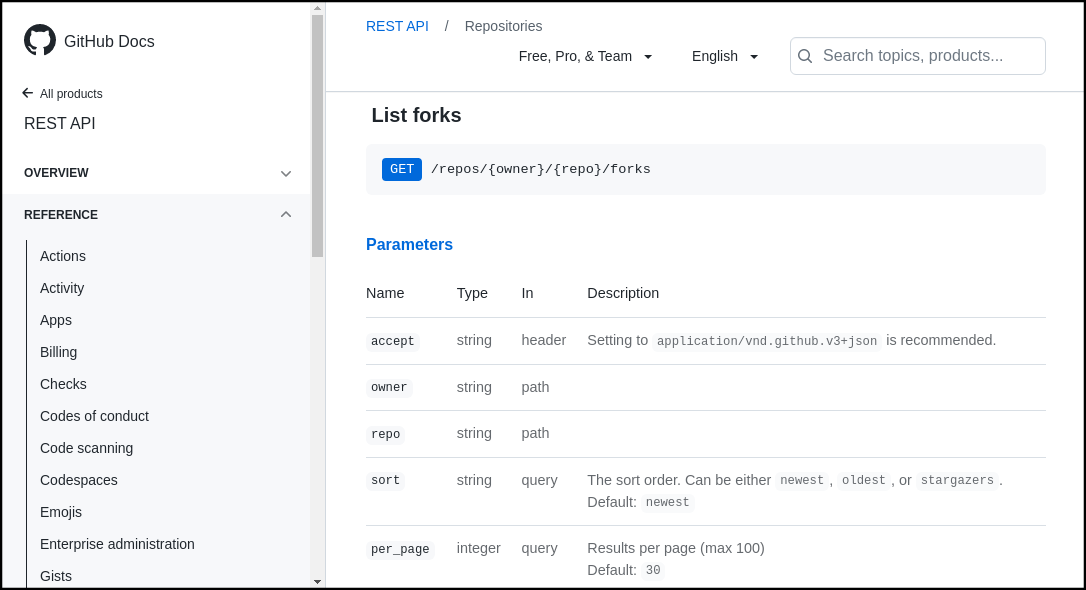
\includegraphics[width=0.5\linewidth]{github-api-website.png}
\end{center}
\end{frame}

\begin{frame}{\only<1-2>{Language use: C++, Python, and Jupyter}\only<3-4>{Packages: ROOT, Scientific Python, Uproot/Awkward}}
\vspace{0.25 cm}
\textcolor{darkblue}{\mbox{\hspace{-0.5 cm}}\only<1-2>{Number of non-fork GitHub repos created by CMS physicists}\only<3-4>{Same sample, now counting matches for \mintinline{python}{import XYZ}, \mintinline{python}{from XYZ import}, etc.}}

\vspace{-0.35 cm}
\begin{columns}
\column{1.15\linewidth}
\only<1>{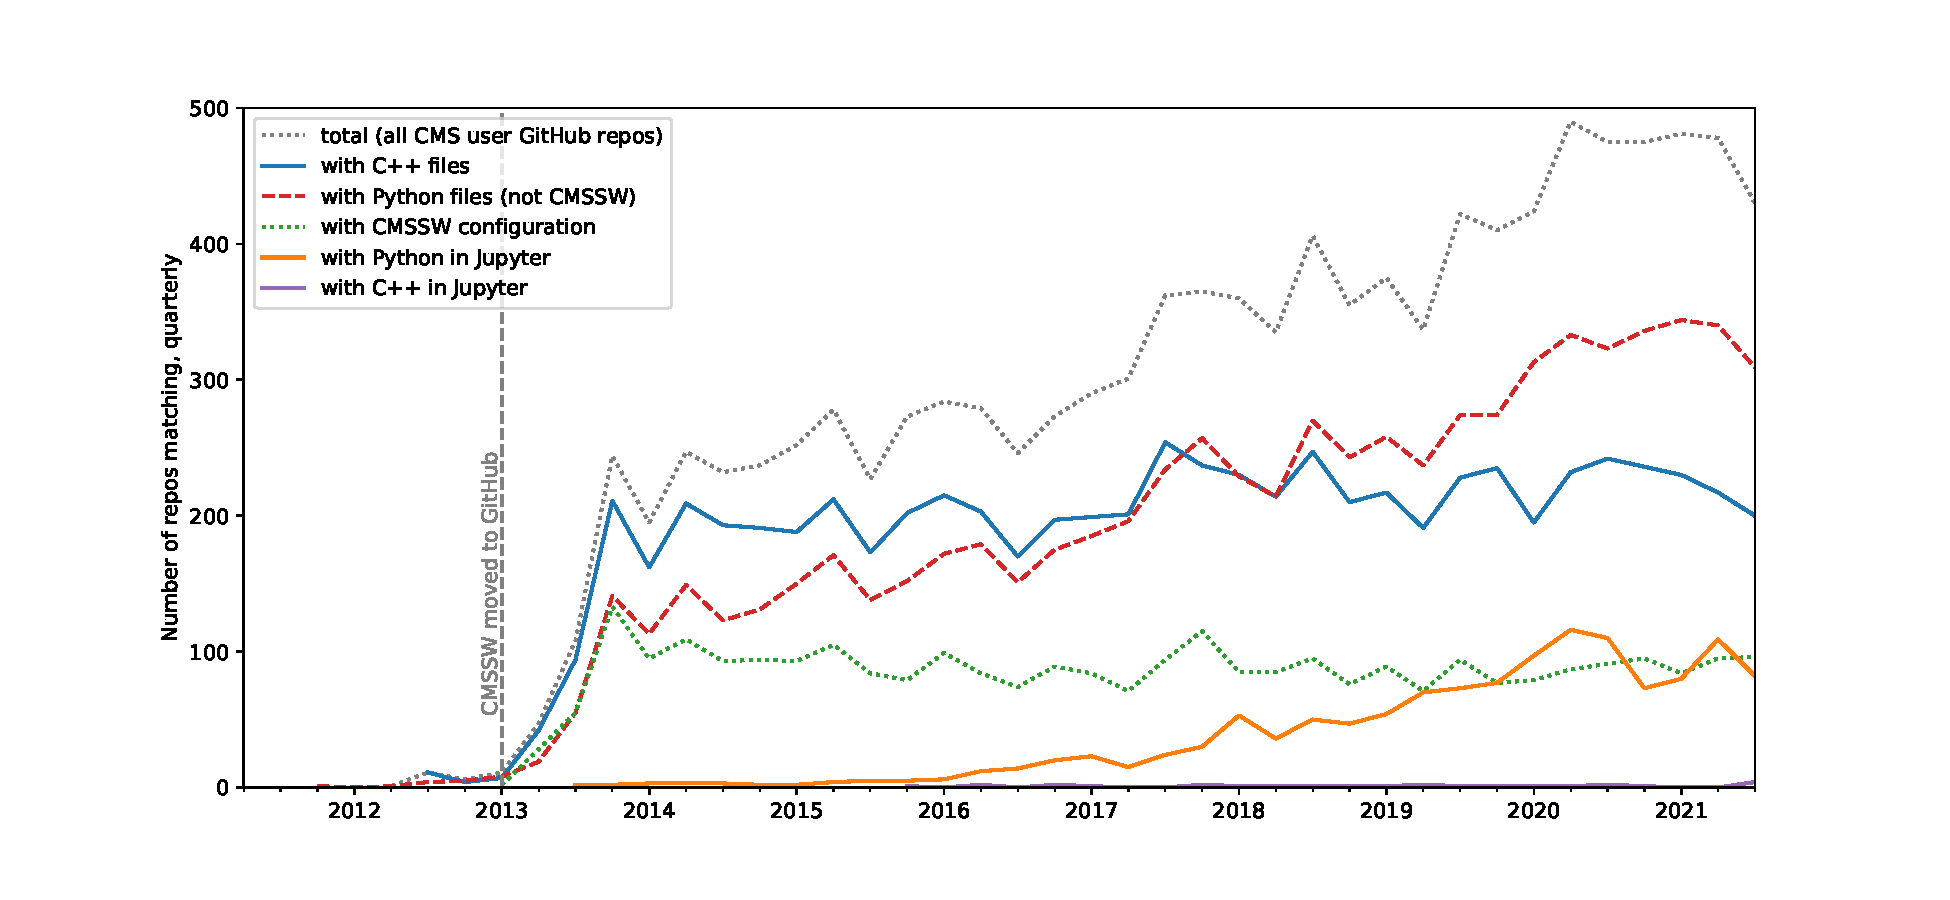
\includegraphics[width=\linewidth]{gihub-language-fullstudy.pdf}}\only<2>{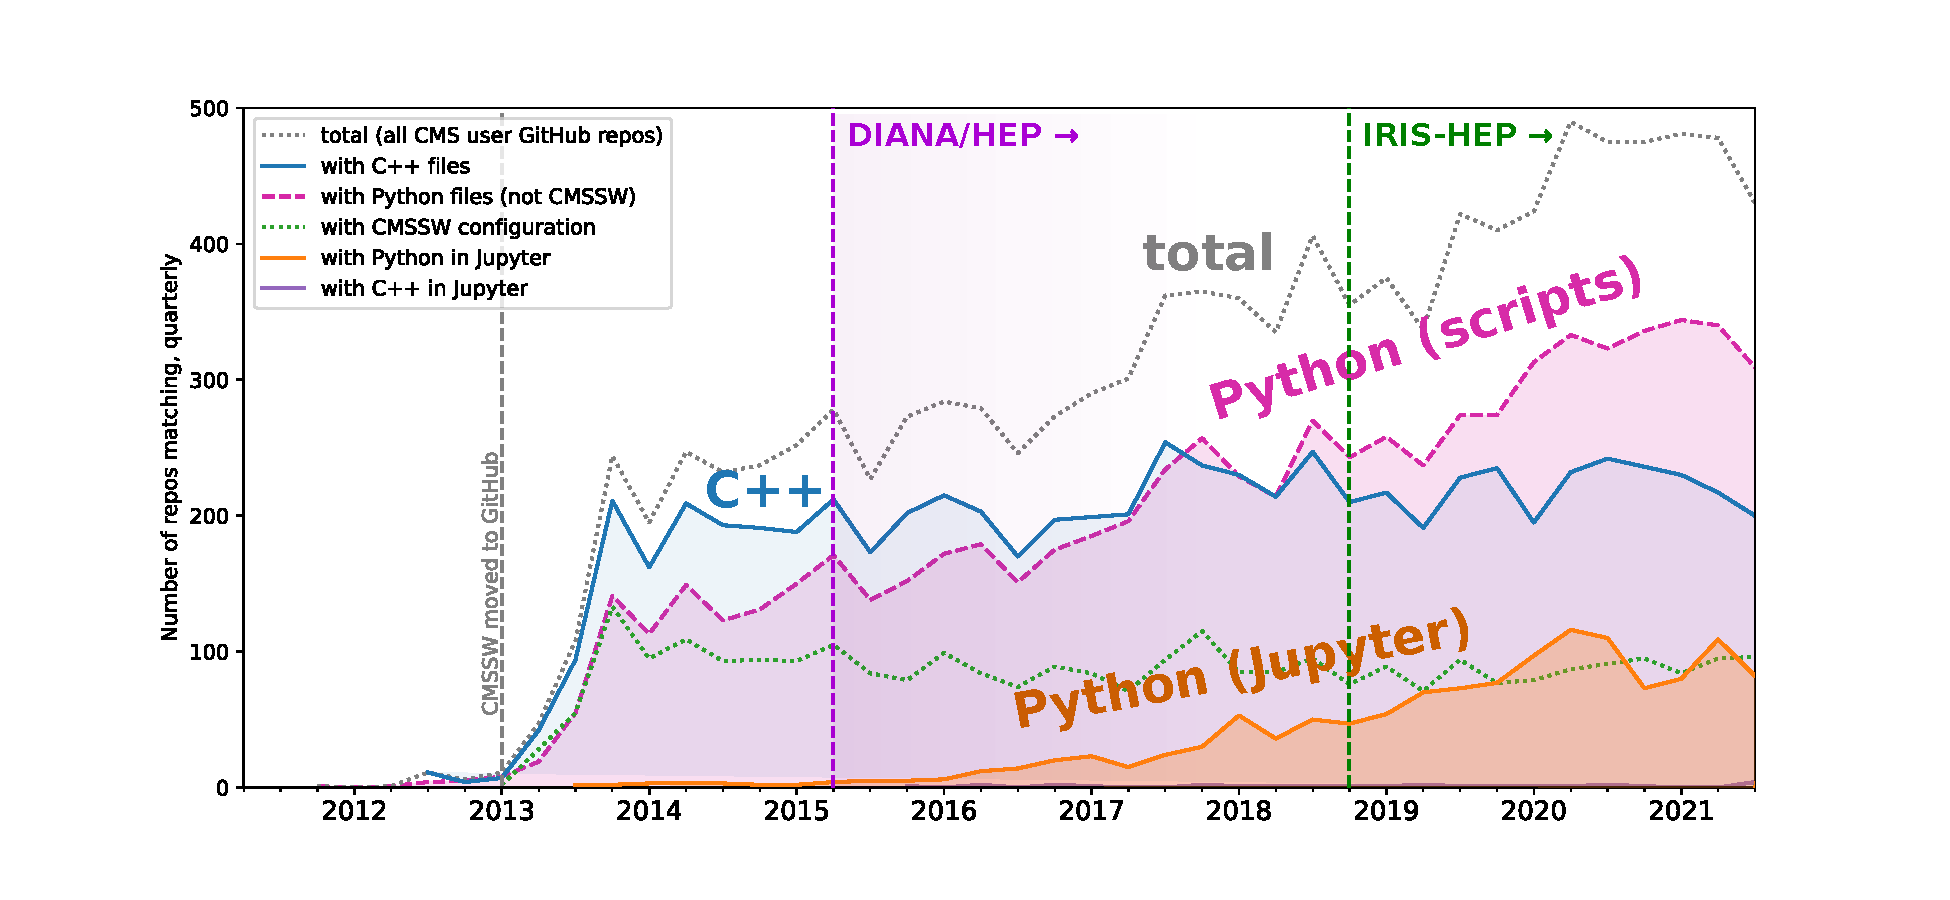
\includegraphics[width=\linewidth]{gihub-language-fullstudy-for-review.pdf}}\only<3>{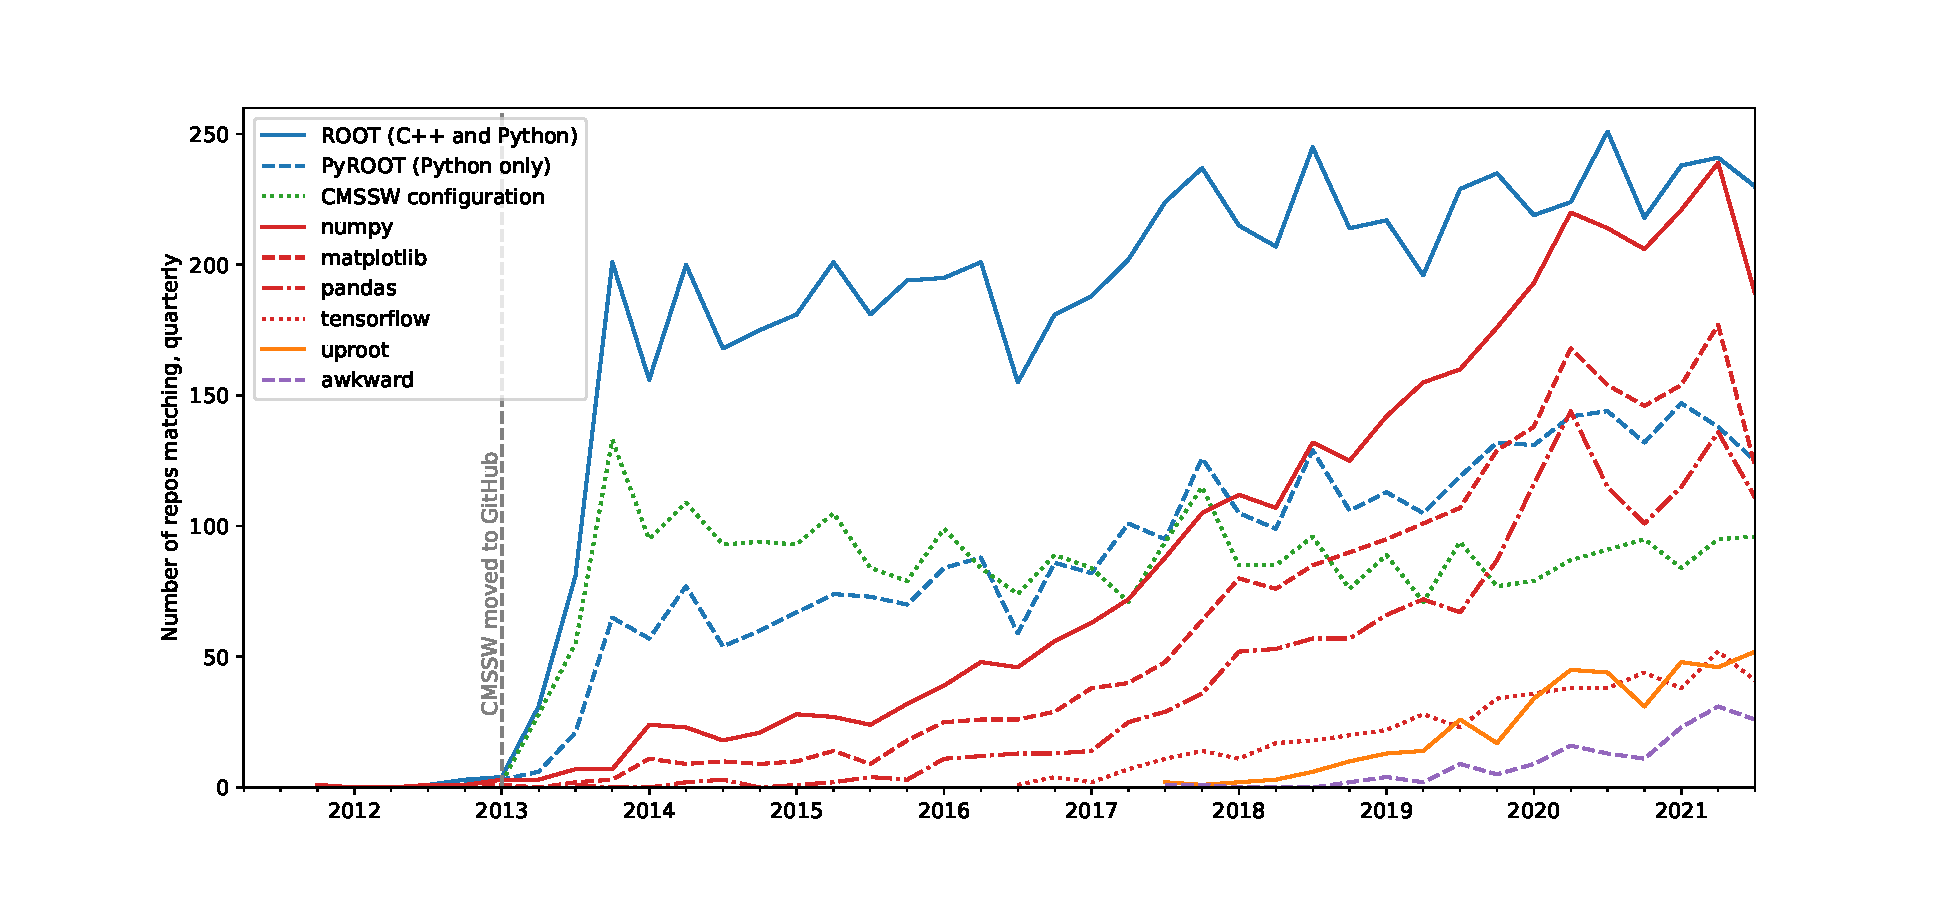
\includegraphics[width=\linewidth]{gihub-package-fullstudy.pdf}}\only<4>{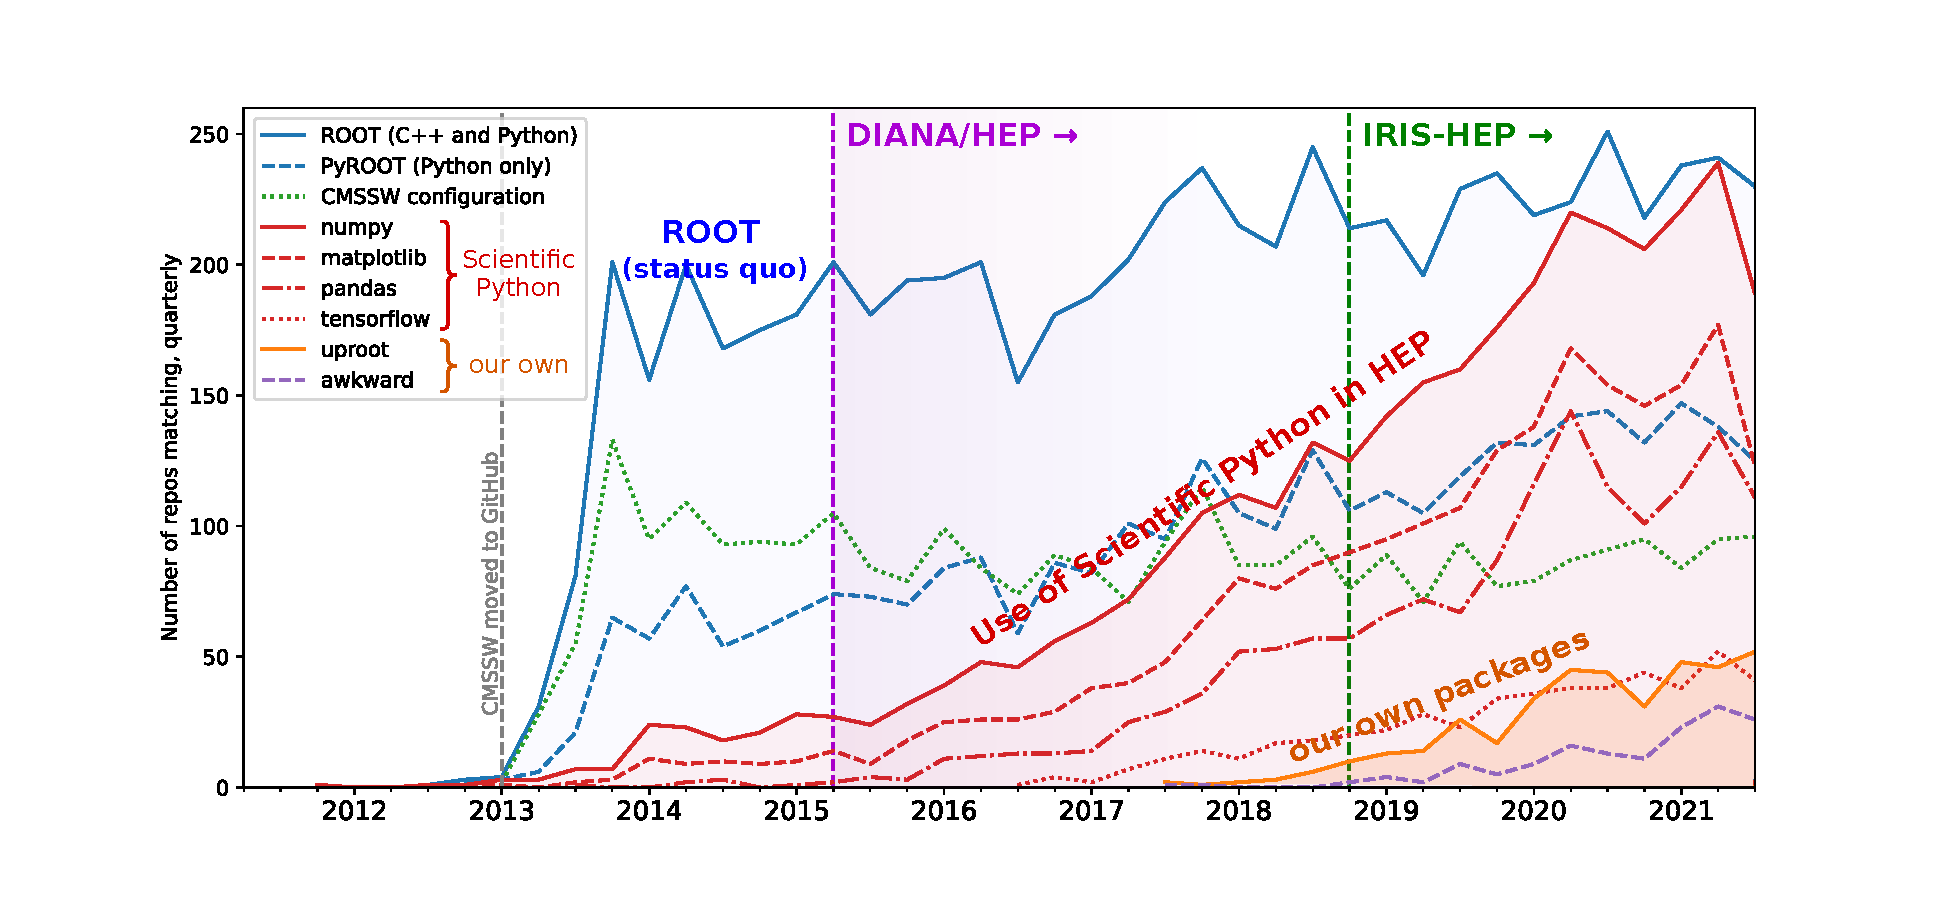
\includegraphics[width=\linewidth]{gihub-package-fullstudy-for-review.pdf}}
\end{columns}
\end{frame}

%% \begin{frame}{This is an update of my earlier GitHub-CMSSW study}
%% \vspace{0.5 cm}
%% \large

%% \begin{enumerate}\setlength{\itemsep}{0.35 cm}
%% \item Inclusively counting ``repo that contains a C++ file'' or ``a Python file,'' rather than GitHub's exclusive determination of ``repo language.''

%% \item Distinguishing between Python files that are CMSSW configurations and other Python files (GitHub doesn't).

%% \item I've downloaded all the repos, so I can run my own regex searches, rather than relying on GitHub's.
%% \end{enumerate}

%% \vspace{0.5 cm}
%% \begin{uncoverenv}<2->
%% We can do more: run clang-tidy/pylint? Features of libraries used?

%% \textcolor{blue}{\scriptsize\url{https://pivarski-princeton.s3.amazonaws.com/GitHub-CMSSW-user-nonfork-raw-data.tar}}

%% \vspace{0.5 cm}
%% \textcolor{gray}{\normalsize (Note: these are all public repos/public data.)}
%% \end{uncoverenv}
%% \end{frame}

\begin{frame}{Longer baseline: title/abstract matches in InspireHEP}
\vspace{0.5 cm}
\begin{itemize}
\item CHEP and ACAT are the two major conferences for computing in HEP.
\item CHEP started in 1985 and includes 5\,407 proceedings.
\item ACAT started in 1990 and includes 1\,446 proceedings.
\item Search all the titles and abstracts for interesting keywords!
\end{itemize}

\vspace{0.25 cm}
\begin{center}
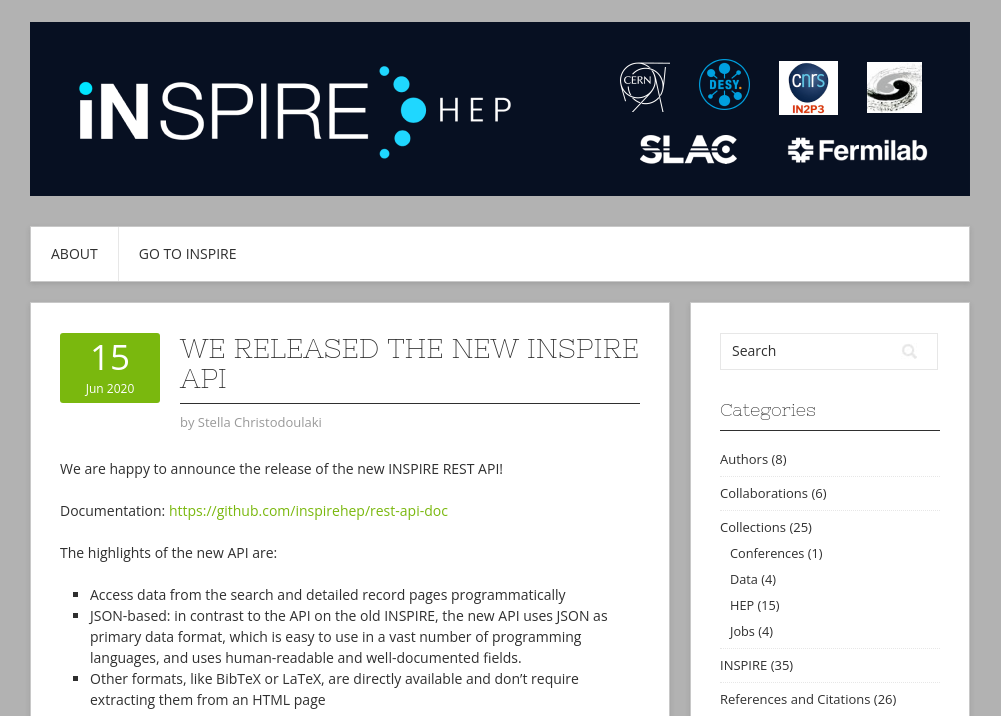
\includegraphics[width=0.5\linewidth]{inspirehep-api-website.png}
\end{center}
\end{frame}

\begin{frame}{Machine learning in \only<1>{CHEP}\only<2>{ACAT} papers}
\vspace{0.35 cm}

\begin{columns}
\column{1.05\linewidth}
\only<1>{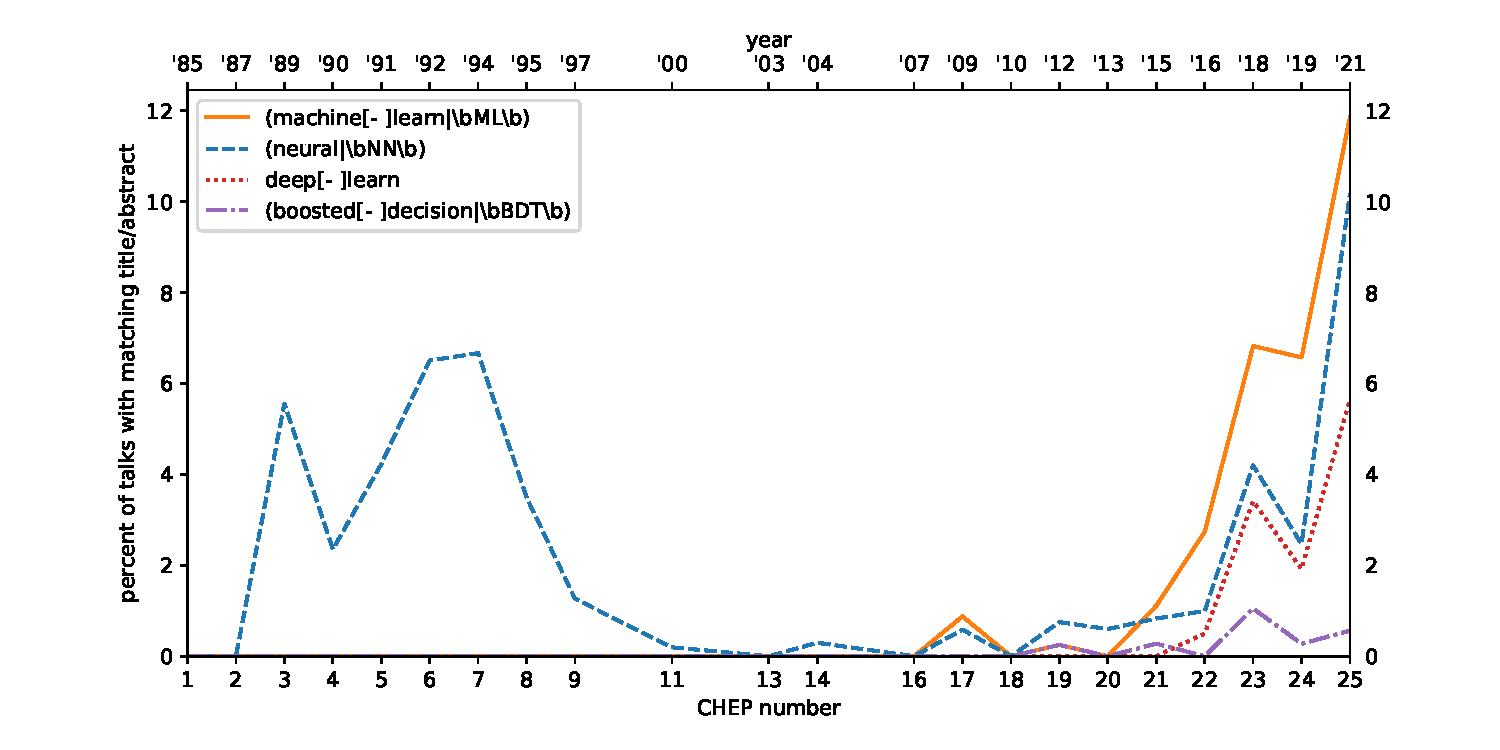
\includegraphics[width=\linewidth]{chep-papers-ml.pdf}}\only<2>{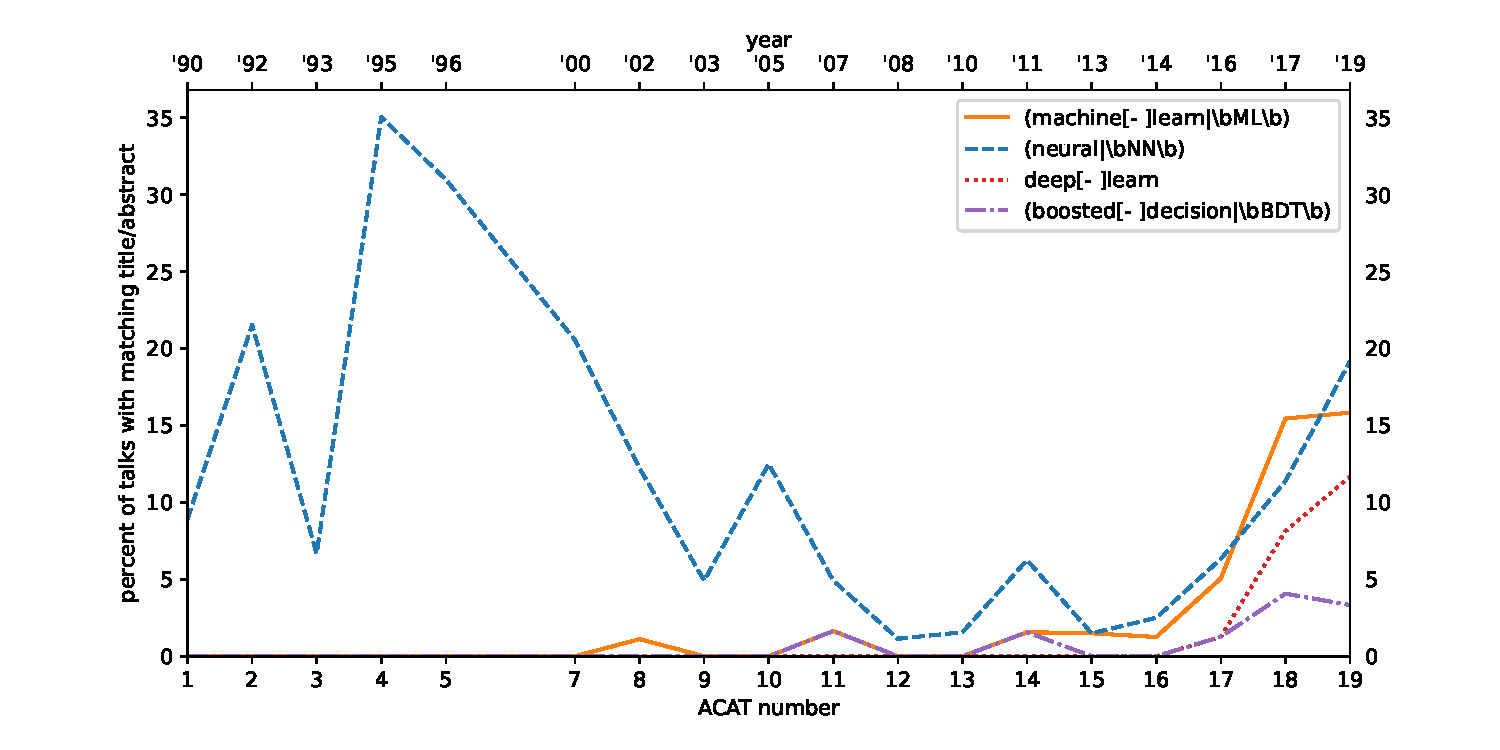
\includegraphics[width=\linewidth]{acat-papers-ml.pdf}}
\end{columns}
\end{frame}

\begin{frame}{Hardware accelerators in \only<1>{CHEP}\only<2>{ACAT} papers}
\vspace{0.35 cm}

\begin{columns}
\column{1.05\linewidth}
\only<1>{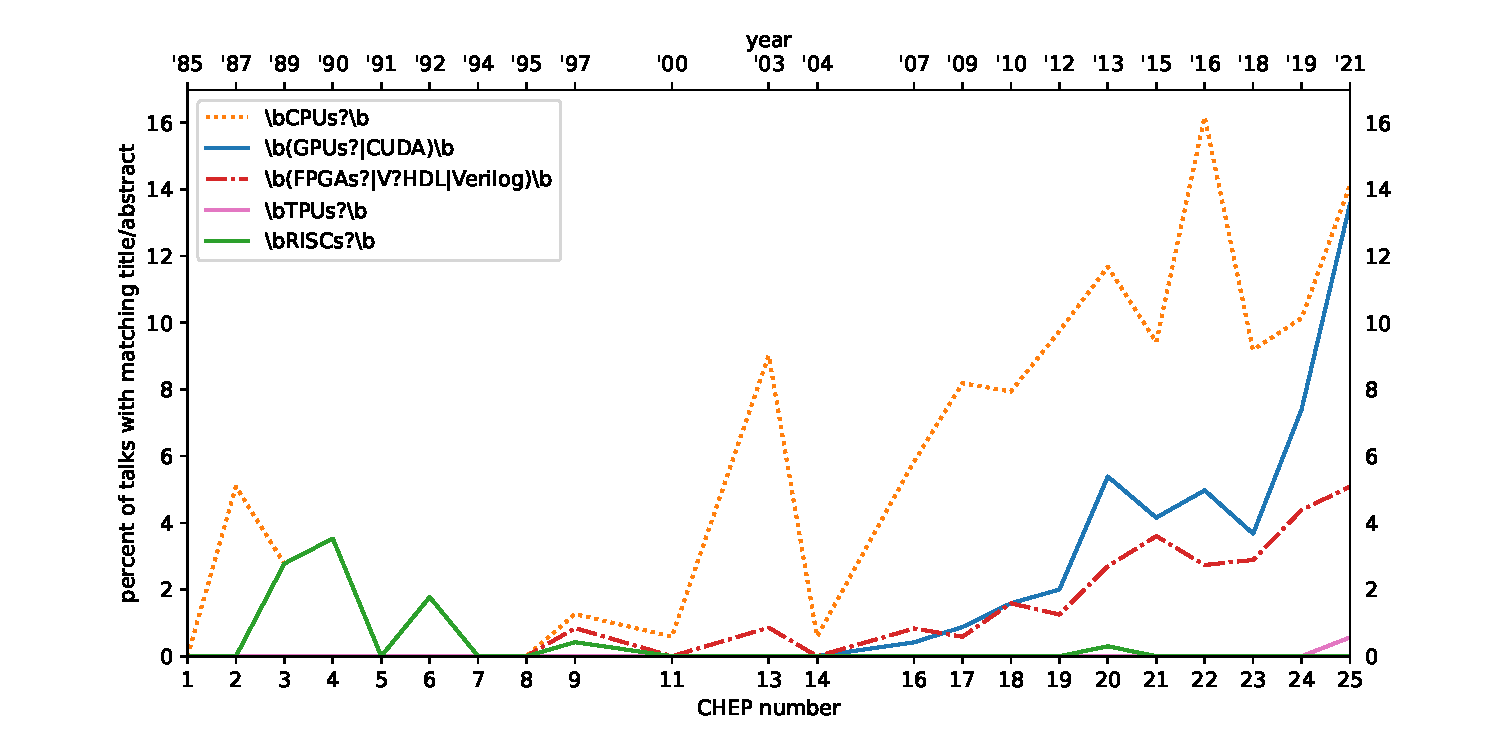
\includegraphics[width=\linewidth]{chep-papers-accelerator.pdf}}\only<2>{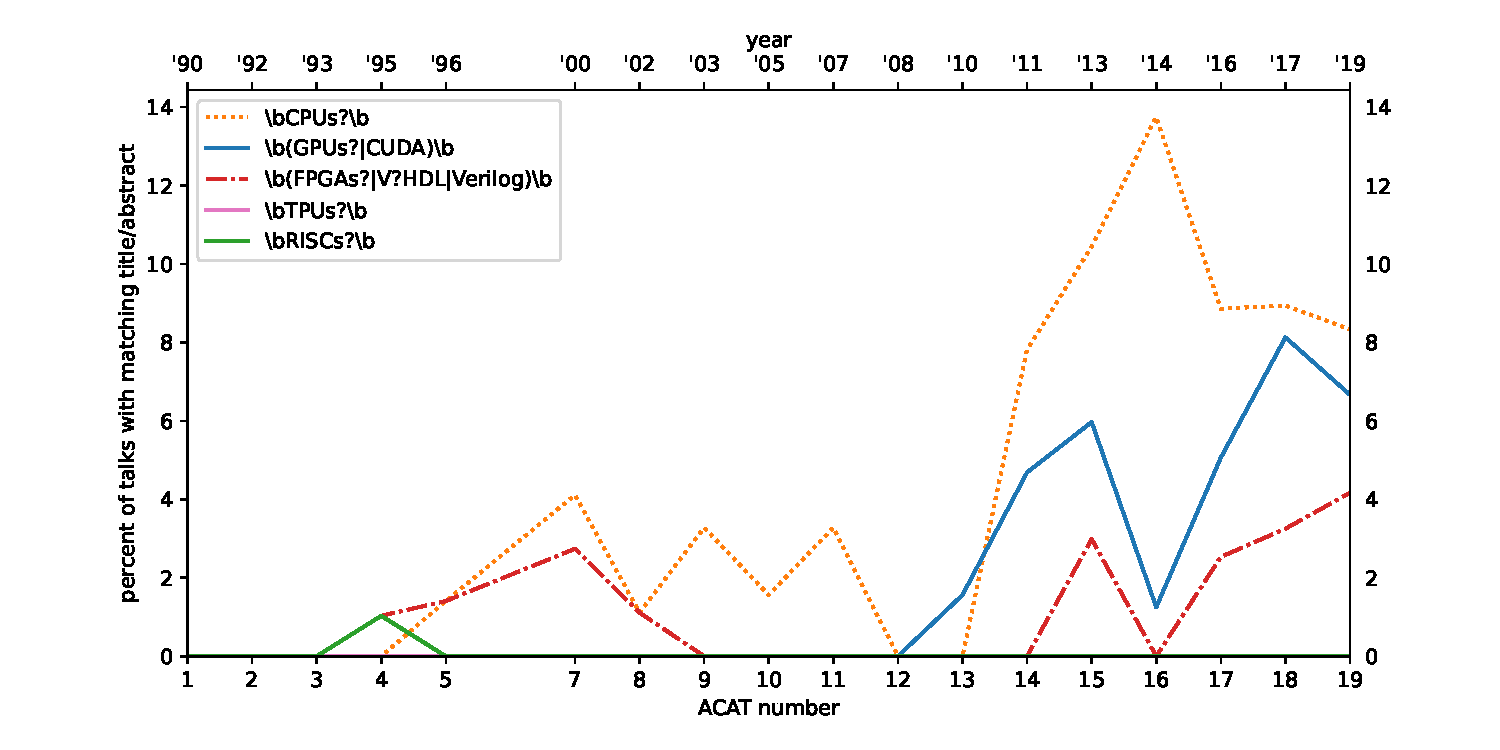
\includegraphics[width=\linewidth]{acat-papers-accelerator.pdf}}
\end{columns}
\end{frame}

\begin{frame}{\mbox{ }}
\vspace{1 cm}
\begin{center}
\Large What about language transitions? Fortran $\to$ C++ $\to$ Python?
\end{center}
\end{frame}

\begin{frame}{Programming languages in \only<1>{CHEP}\only<2>{ACAT} papers}
\vspace{0.35 cm}

\begin{columns}
\column{1.05\linewidth}
\only<1>{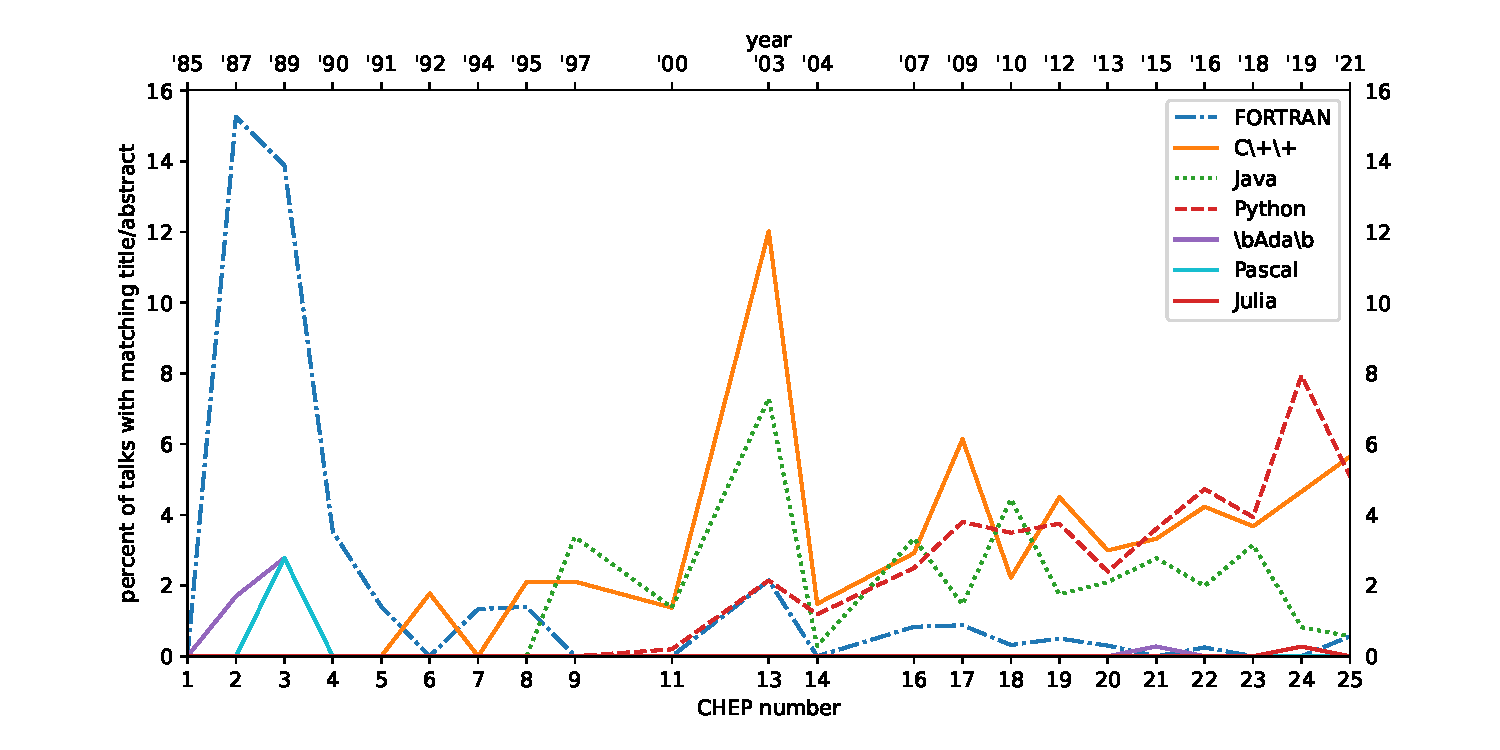
\includegraphics[width=\linewidth]{chep-papers-language.pdf}}\only<2>{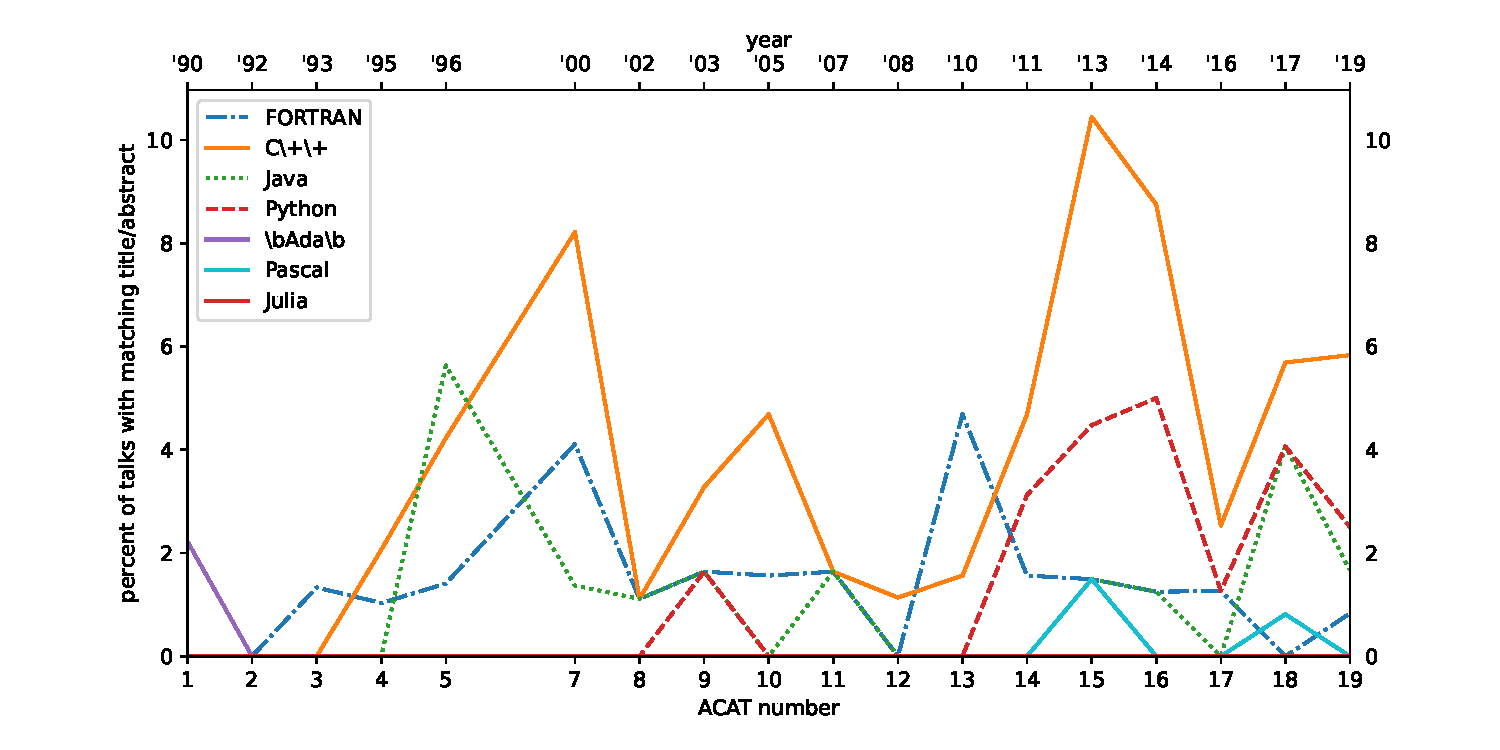
\includegraphics[width=\linewidth]{acat-papers-language.pdf}}
\end{columns}
\end{frame}

\begin{frame}{Lucas Taylor, {\it Summary of Data Analysis Track,} CHEP 2001}
\vspace{0.25 cm}
\begin{columns}
\column{0.05\linewidth}

\column{0.81\linewidth}
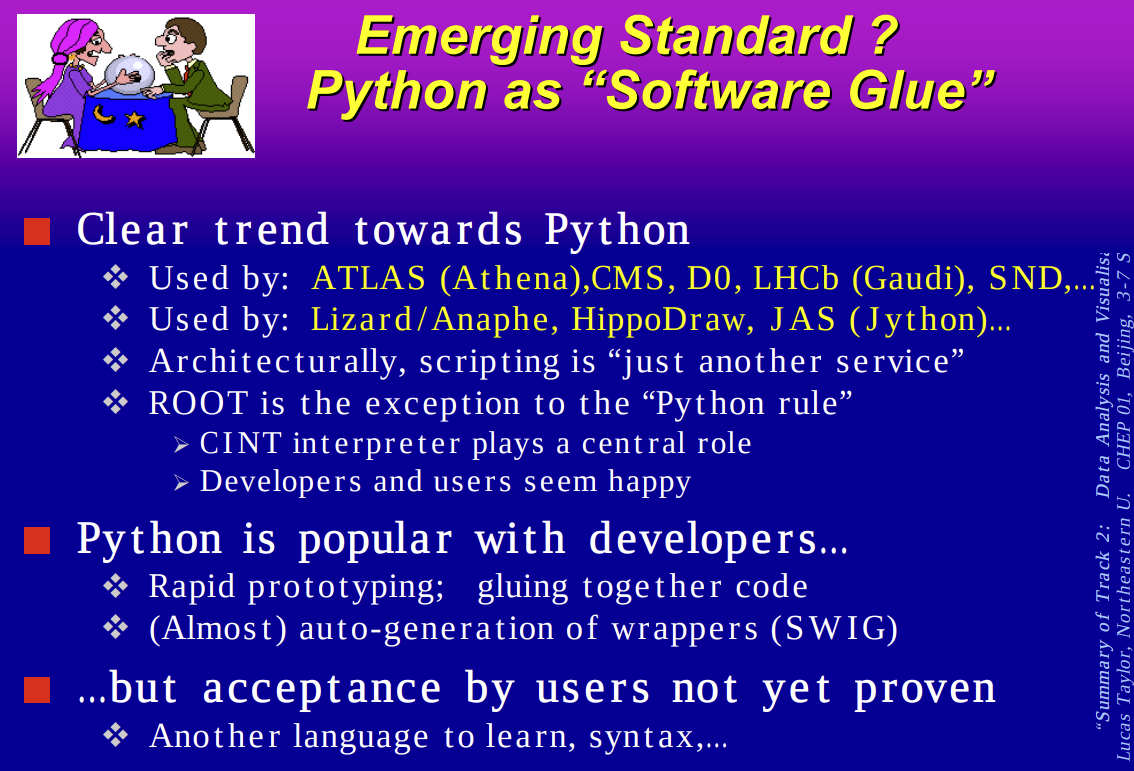
\includegraphics[width=\linewidth]{chep-2001-python.png}

\column{0.2\linewidth}
Note: PyROOT introduced in 2004 (v4.00/04).
\end{columns}
\end{frame}

\begin{frame}{Programming paradigms in \only<1>{CHEP}\only<2>{ACAT} papers}
\vspace{0.35 cm}

\begin{columns}
\column{1.05\linewidth}
\only<1>{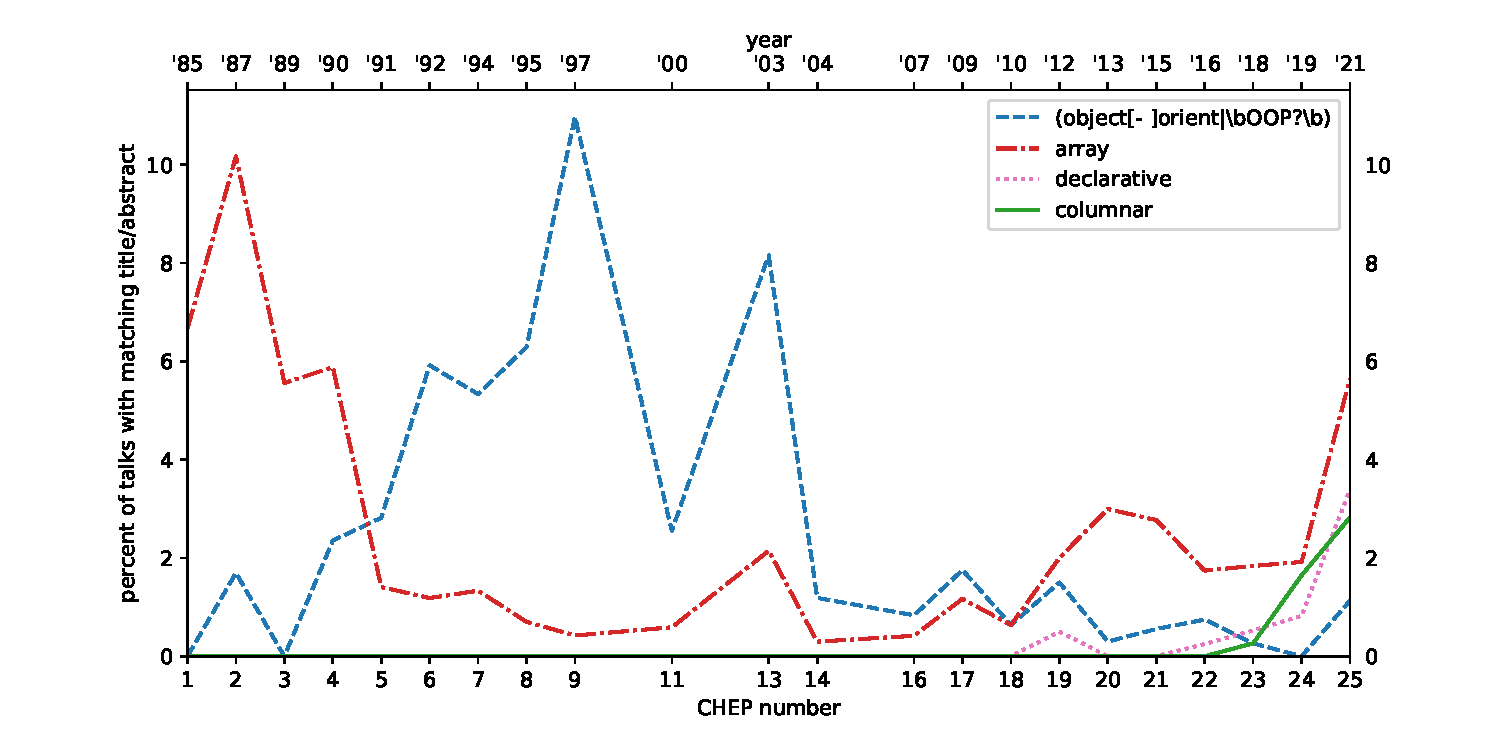
\includegraphics[width=\linewidth]{chep-papers-paradigm.pdf}}\only<2>{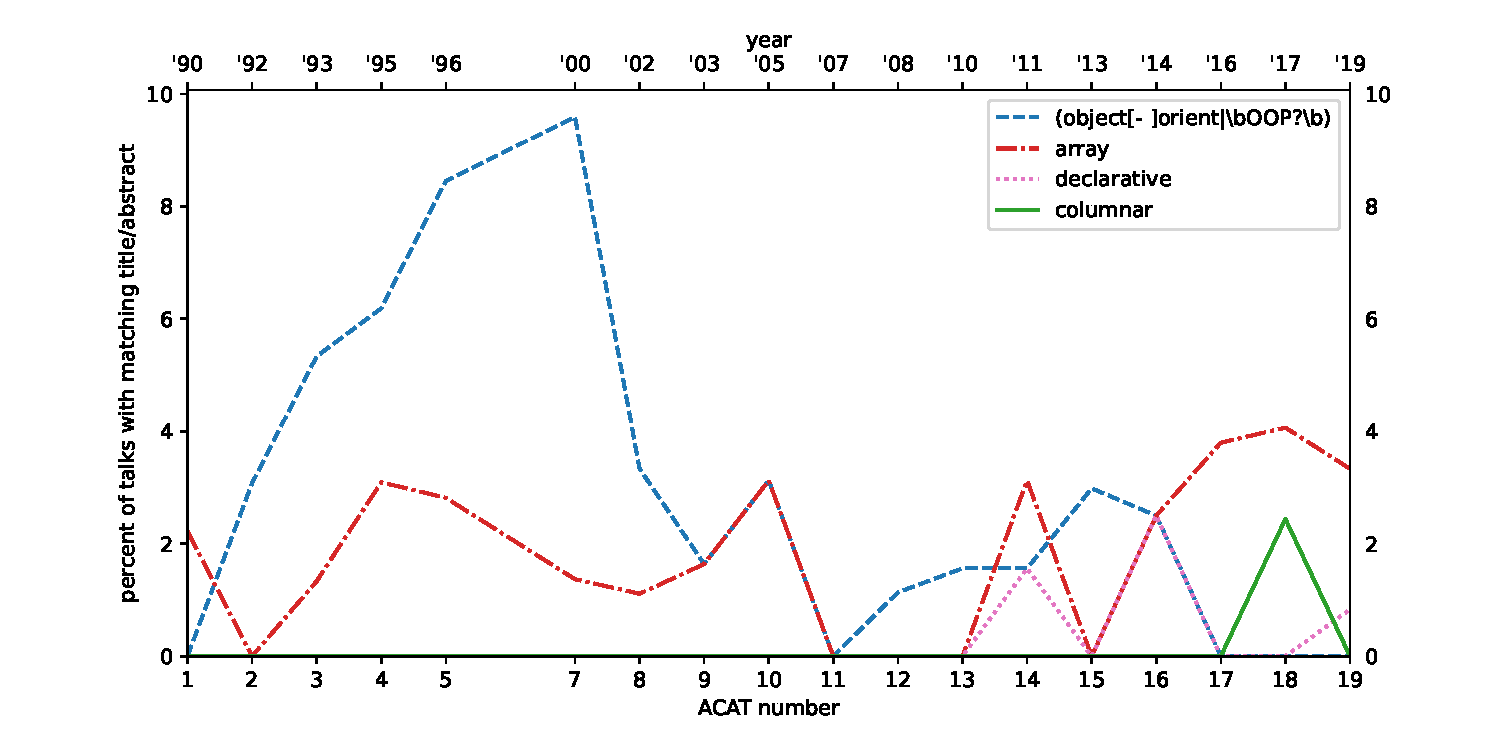
\includegraphics[width=\linewidth]{acat-papers-paradigm.pdf}}
\end{columns}
\end{frame}

\begin{frame}{Software frameworks in \only<1>{CHEP}\only<2>{ACAT} papers}
\vspace{0.35 cm}

\begin{columns}
\column{1.05\linewidth}
\only<1>{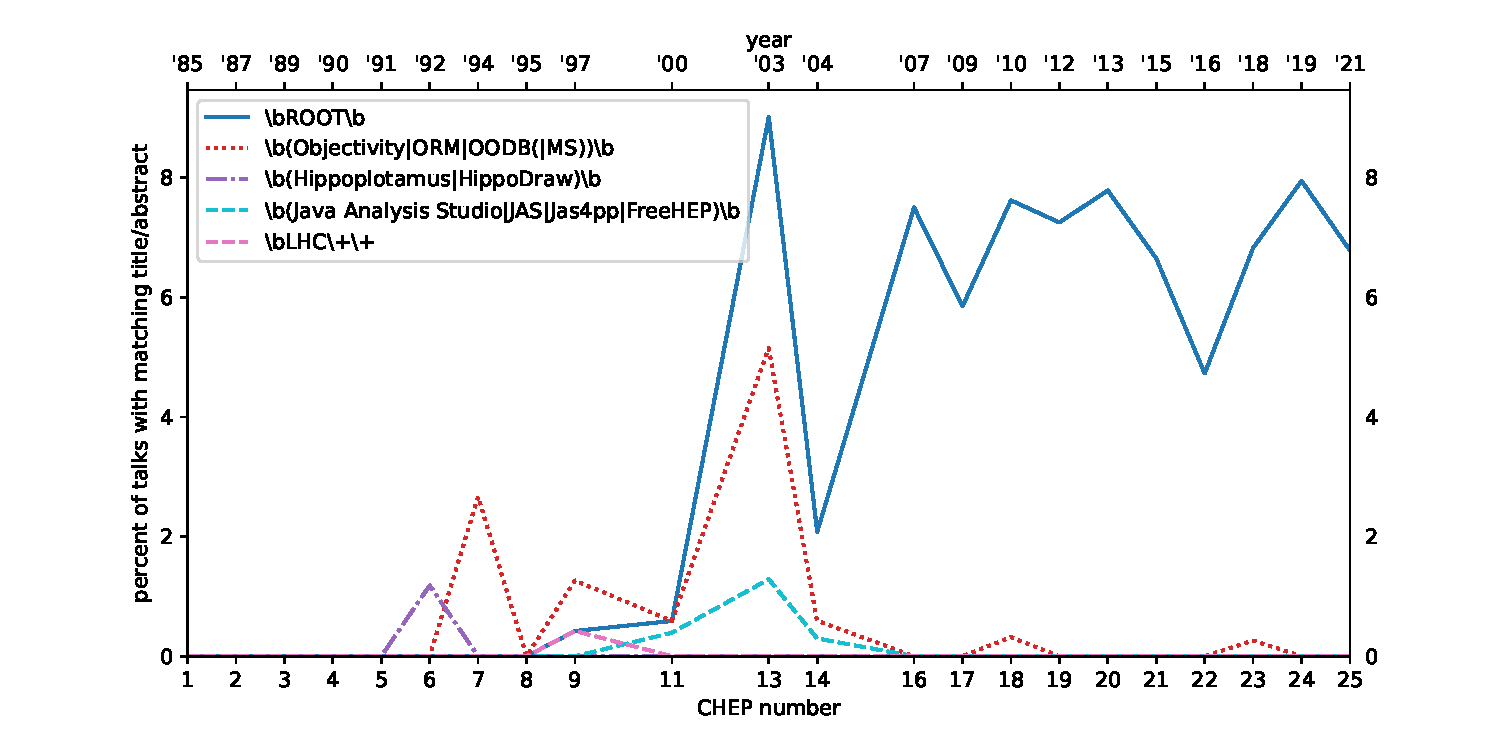
\includegraphics[width=\linewidth]{chep-papers-package-1.pdf}}\only<2>{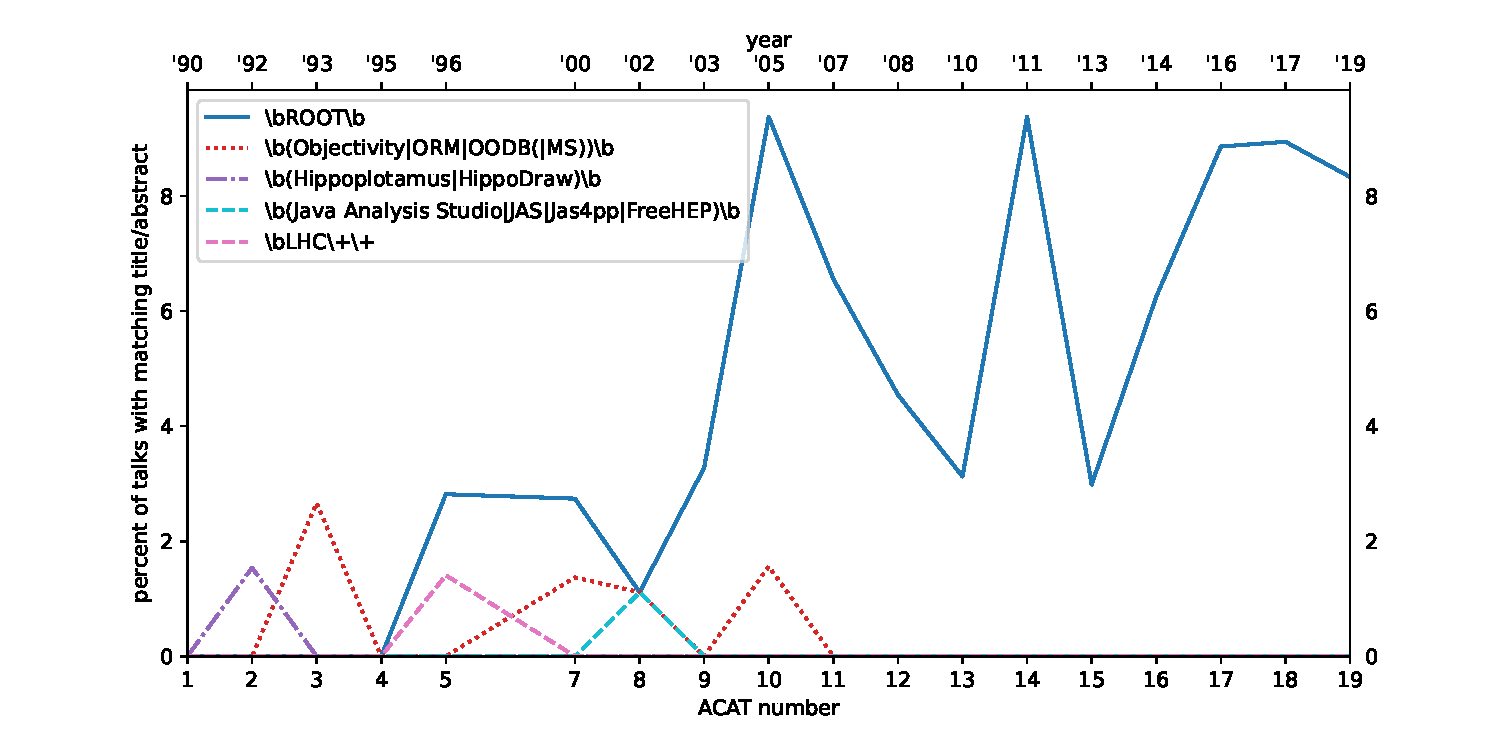
\includegraphics[width=\linewidth]{acat-papers-package-1.pdf}}
\end{columns}
\end{frame}

\begin{frame}{Kinds of tasks in \only<1>{CHEP}\only<2>{ACAT} papers}
\vspace{0.35 cm}

\begin{columns}
\column{1.05\linewidth}
\only<1>{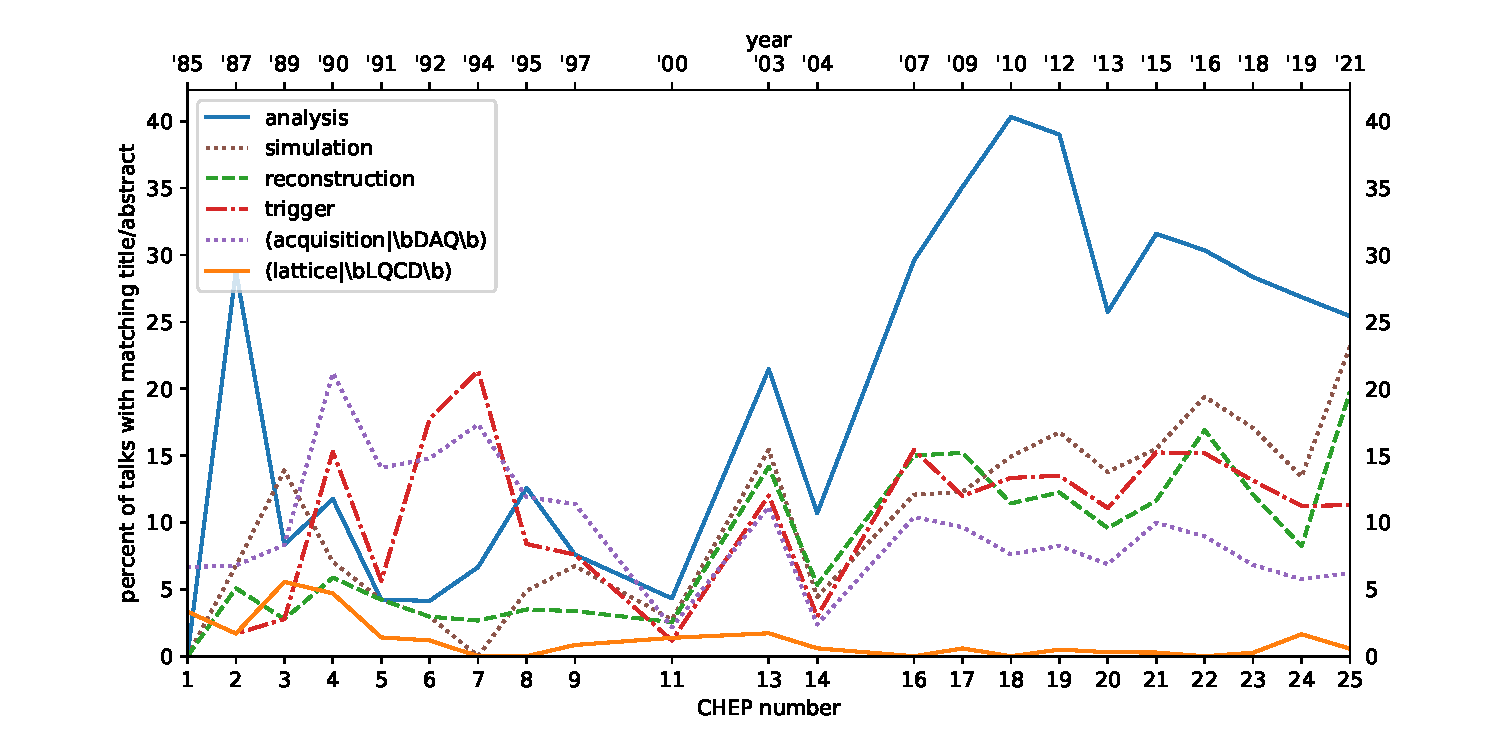
\includegraphics[width=\linewidth]{chep-papers-task.pdf}}\only<2>{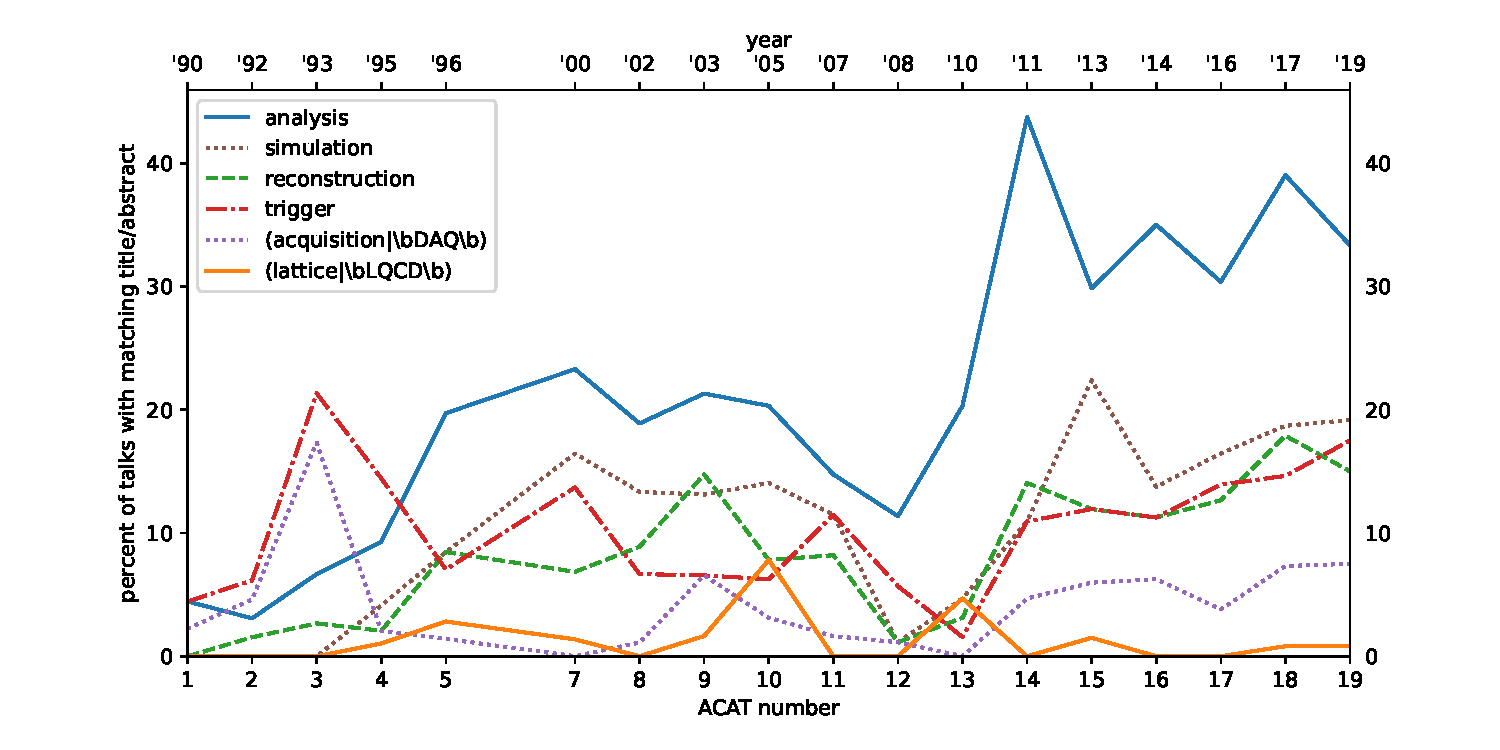
\includegraphics[width=\linewidth]{acat-papers-task.pdf}}
\end{columns}
\end{frame}

\begin{frame}{Conclusions}
\Large
\vspace{0.5 cm}
\begin{itemize}\setlength{\itemsep}{0.5 cm}
\item Different ways of understanding people, including the HEP software community: focus groups, interviews, historical documents, surveys, and proxy metrics.

\item This talk focused on proxy metrics, which are quantitative, but you have to pay close attention to what they're quantifying.

\item Some clear trends and conclusions emerged. \mbox{Others are muddled.\hspace{-1 cm}}
\end{itemize}
\end{frame}

\end{document}
